%\documentclass[compressed,notitlepage,narroweqnarry,inline,12pt,onecolumn]{IEEEtran}
\documentclass[10pt,journal,executivepaper]{IEEEtran}
%\usepackage{latex8}
\usepackage{times}
\usepackage{amssymb}
\usepackage{amsmath}
\usepackage{graphicx}
\usepackage{epstopdf}
\usepackage{subfigure}
\usepackage[nocompress]{cite}
\usepackage{algorithm}
\usepackage{algorithmic}
\usepackage{titlesec}
\usepackage{multirow}
\usepackage{tabularx}
\usepackage{booktabs}
\usepackage{threeparttable}
\usepackage[normalem]{ulem}
\usepackage{url}
\usepackage{CJK}
\pagestyle{plain}
\usepackage{geometry}
\geometry{left=0.5in,right=0.5in,top=0.5in,bottom=0.5in}
%%\geometry{left=1.40cm,right=1.40cm,top=1.33cm,bottom=2.1cm}
%%\linespread{0.986}
%\setlength{\abovedisplayskip}{1 mm}
%\setlength{\belowdisplayskip}{0.5 mm}
%%\setlength{\abovecaptionskip}{0.0pt}
%%\setlength{\belowcaptionskip}{0.0pt}
%%\titlespacing{\section}{0pt}{4pt}{0 pt}
%%\titlespacing{\subsection}{0pt}{2pt}{0pt}
%%\titlespacing{\subsubsection}{0pt}{2pt}{0pt}

\usepackage[colorlinks,linkcolor=red,anchorcolor=blue]{hyperref}
\newcommand{\rev}[1]{\uwave{#1}}
%\newcommand{\rev}[1]{#1}
\renewcommand{\algorithmicrequire}{\textbf{Input:}}
\renewcommand{\algorithmicensure}{\textbf{Output:}}

\newcommand{\del}[1]{\sout{#1}}  %revise the text
%\newcommand{\del}[1]{}

\newcommand{\note}[1]{{\sffamily\itshape\bfseries\uline{#1}}}


\newcommand{\DataSetSize}{$3 \times 10^6$ }
\newcommand{\SearchDataSize}{$5 \times 10^5$ }
\newcommand{\SecIXone}{$x$}
\newcommand{\SecIXtwo}{$x$}

\begin{document}
\title{SFBF: Scalable and Flexible Bloom Filter for Ever-increasing Big Data}
\author{Kun Xie$^1$, \emph{Member, IEEE}, Heng Tao$^1$, Xin Wang$^1$, \emph{Member, IEEE},  Jigang Wen$^2$, \\ Yinghua Min$^2$, \emph{Fellow, IEEE},  Keqin Li$^3$ \emph{Fellow, IEEE},  Gaogang Xie$^2$, \emph{Member, IEEE}\\
$^1$ Department of Electrical and Computer Engineering, State University of New York at Stony Brook, USA\\
$^2$ Institute of Computing Technology, Chinese Academy of Sciences, Beijing 100191, China\\
$^3$ Department of Computer Science, State University of New York, New Paltz, NY 12561, USA\\
%$^3$ School of Information Science and Engineering, Hunan University, Changsha 410082, China\\
kun.xie@stonybrook.edu, franztaoheng@gmail.com, x.wang@stonybrook.edu,  wenjigang@ict.ac.cn,  \\ min@ict.ac.cn, lik@newpaltz.edu, xie@ict.ac.cn}
\maketitle
\vspace{-3em}
%\vspace{-0.6in}
\begin{abstract}
Bloom filters (BF) allow membership queries over sets with allowable error rate. It is widely used in databases, networks and distributed systems. Despite that BF can work well to represent a static data set by optimally setting the BF parameters to achieve a low false positive rate based on the data set size, when there are dynamic data arrivals thus constant data set changes, it would lead to high false positive errors in BF. To make BF scalable, we propose a Scalable and Flexible Bloom filter (SFBF) to control the false positive rate at a low level even when there are ever-increasing data arrivals and the size of the data set is unpredictable. Specifically, we propose a novel algorithm to adaptively generate hash functions and a light-weight SFBF query algorithm that takes advantage of the features of our proposed hash functions to provide quick BF query. Our performance results demonstrate that SFBF offers very good performance (low false positive rate and low query time) in the presence of dynamic data arrivals, even when the data set becomes very large.
\end{abstract}


\section{Introduction}

Recently, various applications such as information retrieval, telecommunications, transaction records, network monitoring have generated a large amount of data, which makes the data intensive computing a major area of interest both in the industry and in the research community. Efficient storage, management, and processing of the massive amount of data are important and challenging.

As a space efficient probabilistic data structure, Bloom filter (BF) \cite{bloom1970space} can support the set membership query with a low probability of false positive (i.e., falsely identifying an element to be a member of the set while it is not), no false negative, as well as efficiency in query and storage. The simplicity, easiness
of use, straightforward mapping to hardware, and excellent
performance (low false positive rate and $O(1)$ update complexity) make Bloom Filter attractive for many applications,
especially for applications in distributed systems to share
information about available data \cite{Broder2004,tarkoma2012theory}.

However, with unpredicted large scale and ever-increasing data, there is a big challenge to design an efficient and scalable Bloom filter.
Despite the fact that BF can work well to represent a static data set where BF parameters are set to achieve a low false positive rate for a fixed size data set, there are many practical challenges to apply the conventional BF in the presence of "Big Data" for the following reasons:


First, the growth of data set will result in higher false positive rate if the conventional BF is applied for membership query. Dynamically expanding the BF size is an option to solve this problem, however, it needs a well-designed expanding rule to control the false positive rate at low level.

Second, with the size change of the BF, it introduces the need and challenge to find the hash functions that can obtain the hash values within the new BF range at low overhead.

Third, to quickly find the membership of an element in a big data set, it is critical to ensure light-weight BF matching to determine if the set contains the data item. The variations of the BF size and hash functions introduce additional challenge for quick data query.

Although several BF variants \cite{6848046,fan2000summary,mitzenmacher2002compressed,kumar2006space,deng2006approximately,dutta2012towards,dutta2013streaming,yoon2010aging,tree6848077,guo2006theory, xie2007scalable} have been proposed in the literature to suit
various application needs to reduce the information processing and memory/bandwidth cost,
among which, only a very few Bloom filters \cite{guo2006theory, wei2010mad2,almeida2007scalable,xie2007scalable} have investigated the scalable problem. However, due to the use of static expanding rule or the lack of adaptive hash function design, existing solutions can be hardly  applied in practical network environment.

To address these challenging issues for BF to function efficiently in the presence of large and varying data set, we propose a Scalable and Flexible Bloom filter (SFBF) infrastructure to achieve high matching accuracy with low false positive rate. SFBF can control the false positive rate at a low level and can achieve very low query time even when the total number of data items is unpredictable and data items arrive dynamically. Our contributions of this work can be summarized as follows:
\begin{itemize}
  \item To represent large scale and ever-increasing data, instead of using a single Bloom filter, we consider the use of a BF set consisting of an array of SFBF vectors, with each BF vector added upon need and the length varied based on the flexible expanding speed.
  \item We propose a novel algorithm to adaptively generate hash functions according to various BF vector length in SFBF. Although multiple BF vectors in SFBF require finding multiple groups of hash values for each data item (one group for one BF vector), in our algorithm, only one group of hash values need to be calculated, from which other groups can be easily deduced through very simple and low cost bit shifting operations.
  \item We develop a light-weight SFBF query algorithm that takes advantage of the features of our proposed hash functions to quickly detect whether an element is in a data set or not. Although SFBF consists of multiple BF vectors, with our well designed hash functions, we can achieve significant computation complexity reduction for testing element in big data.
\end{itemize}


The rest of this paper is organized as follows. We review the related work in Section \ref{sec:RELATED_WORK}. We present the basic BF techniques and  our problem in Section \ref{sec:Review of Bloom filter}. We give an overview of SFBF design in Section \ref{sec:Scalable and rate-dependent bloom filter}, and then describe our algorithms for adaptive hash function generation and light-weight SFBF query in Sections \ref{sec:Adaptive Hash function Generation} and \ref{sec: Low Cost Information Query and Data Maintenance}. In Section \ref{sec:SFBF Analysis}, we analyze the performance of the proposed SFBF. We evaluate the performance of the proposed mechanisms through extensive simulations in Section \ref{sec:simulation}, and conclude the work in Section \ref{sec:CONCLUSION}.



\section{Related work}
\label{sec:RELATED_WORK}
%Duplicate detection becomes one of the most important problems within the domains of databases, and network because it can improve resource utilization and compute efficiency.
%A straightforward solution to solve the quick duplication detection problem is using similar buffering and caching mechanisms to store the raw data in high speed memory. \note{Why would de-duplication be related to data storage, although the technique helps to reducing the data storage? dear sister, i delete data storage.}
% However, since the storage of all data arriving from a stream is infeasible, such mechanisms fails to deal with big data streams. Instead of storing the raw data, storing the summary of the data and approximately estimating the duplication with a tolerable error rate become a feasible solution.
%\note{It is not clear how these is related to the de-duplication. Also, do you mean storing the summary in fast speed memory? Original data will need to be stored somewhere anyway. Dear sister, Yes, store the summary of the data information in fast speed memory rather than a disk can faster the query process. if you think above contents are not very related to our work, I can delete the whole paragraph. So that we can also save the limited space}

As a good summary data structure, Bloom filter (BF) can compactly represent a set and effectively filter out elements not belonging to the set. For various applications to reduce the information processing and memory/bandwidth cost, several BF variants are proposed for quick membership query.
These include, key-value Bloom filter \cite{6848046}, counting Bloom filter \cite{fan2000summary}, compressed Bloom filter \cite{mitzenmacher2002compressed}, spacecode Bloom filter \cite{kumar2006space}, spectral Bloom filter \cite{cohen2003spectral}, stable Bloom filter \cite{deng2006approximately}, reservoir sampling based Bloom filter \cite{dutta2012towards},  streaming quotient filter \cite{dutta2013streaming}, aging Bloom filter \cite{yoon2010aging}, and Bloom tree \cite{tree6848077} among many.
%Counting Bloom filters replace an array of bits with counters in order to count the number of items hashed to a particular location.



%The others use subtle variations to efficiently meet the nature of demand of the applications.

However, the increase of data amount and unpredicted data arrival speed bring big challenges for designing and efficient and scalable bloom filter. Among current Bloom filter variants, to support dynamic data set, counting Bloom filter \cite{fan2000summary}, stable Bloom filter \cite{deng2006approximately}, and aging Bloom filter \cite{yoon2010aging} enable the deletion of old elements from Bloom filter. However, these studies can not be directly applied to solve the scalable problem which is the focus of this paper.


Despite the well-known challenge of applying BF to represent a dynamic set with constant increase of data, only a very limited number of attempts are made to deal with the scalability issue.
 The dynamic Bloom filter (DBF) in \cite{guo2006theory, wei2010mad2} expands the Bloom filter by adding a fixed-size BF vector each time as the set size increases, but the false positive rate increases proportionally with the data set size. Authors in \cite{almeida2007scalable} proposed to add new BF vector with the length $s$ times that of the previous one added. Without modifying and controlling the hash functions to make hash values fall within the new BF vector range, this scheme may fail when the BF length changes.
 %fails to work in a practical BF application.  Lack of accompanied hash function design, this BF design may fail to work when BF length changes.
  In our previous work \cite{xie2007scalable}, we proposed a scheme to keep a low false positive rate by doubling the size of the newly added BF vector each time at the cost of BF space occupancy.  Overall, existing studies expand the BF at the same expanding speed (e.g., 1, 2, and $s$ times), which may fail when the data item arrivals are very dynamic.

In contrast, we design a scalable and flexible Bloom filter (SFBF) with dynamic and flexible expanding speed. We also propose a novel algorithm to adaptively generate hash functions based on the vector length to expand in SFBF, and our specific hash design allows for fast BF matching.

\section{Preliminaries, motivation and problem}
\label{sec:Review of Bloom filter}
In this section, we first introduce the fundamentals of basic Bloom filter, we then present the scalability requirement for ever-increasing big data and our design goal.
\subsection{Basic concept of Bloom filter}
\label{subsec:Basic concept of Bloom filter}
A Bloom filter is used to represent a set $S = \left\{ {{s_1},{s_2}, \cdots ,{s_n}} \right\}$ of $n$ elements from a universe $U$. It can be represented as an $m$ bit vector with elements $BF[0],BF[1], \cdots ,BF\left[ {m - 1} \right]$, initially all set to 0.
In many applications of Bloom filters, the summary message is captured with $m$-bit vector BF and transmitted in the system.
The filter uses $k$ independent hash functions $h_1,h_2, \cdots ,h_k$, with each hash function independently mapping an element in the universe to a random number uniformly over the range ${0,1, \cdots ,m-1}$. For each element ${x} \in {\text{S}}$, the bits $BF[h_i(x)]$ are set to 1 for $1 \le i \le k$, as shown in Fig.\ref{fig:BFinsert}. Given an item $y$, we check its membership by examining the BF whether the bits at positions $h_1(y),h_2(y), \cdots ,h_k(y)$ are set to 1.  If not, then $y$ is definitely not a member of $S$.  If $h_i(y)$ ($1 \le i \le k$) are all set to 1, we assume that $y$ is in $S$, although it can be wrong with some probability. %\rev{which is called {\em false positive rate}}.
%Fig.\ref{fig:Operations on basic bloom filter} shows the operations of the basic Bloom filter.
As every element is hashed into the Bloom filter, the source element can not be observed from the Bloom filter. Therefore, the privacy of the source element is protected.
\begin{figure}[!h]
\centering
\subfigure[Insertion operation]{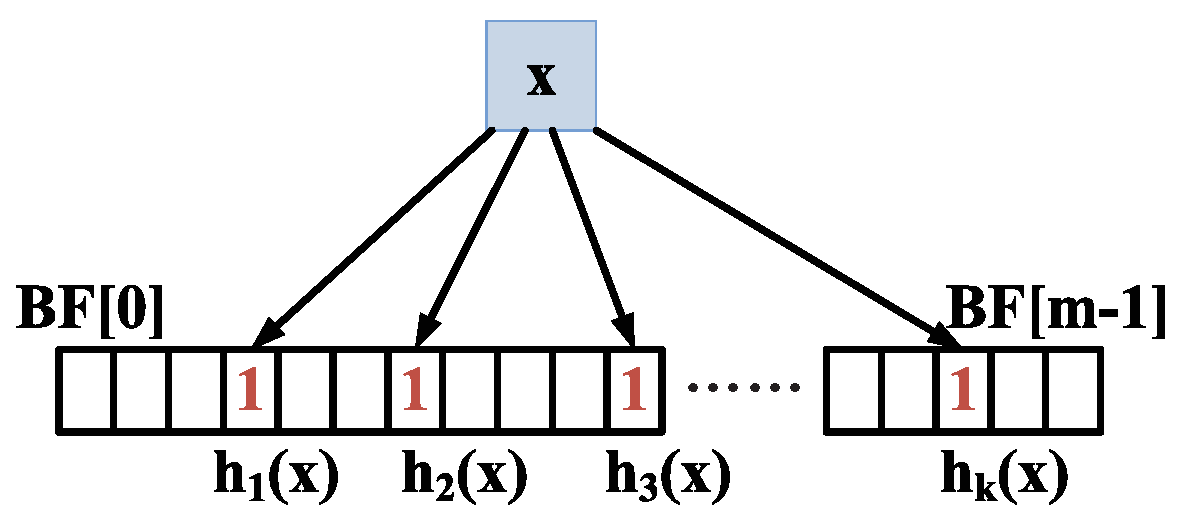
\includegraphics[width=1.4 in]{fig/BFinsert}\label{fig:BFinsert}}
\subfigure[False positive]{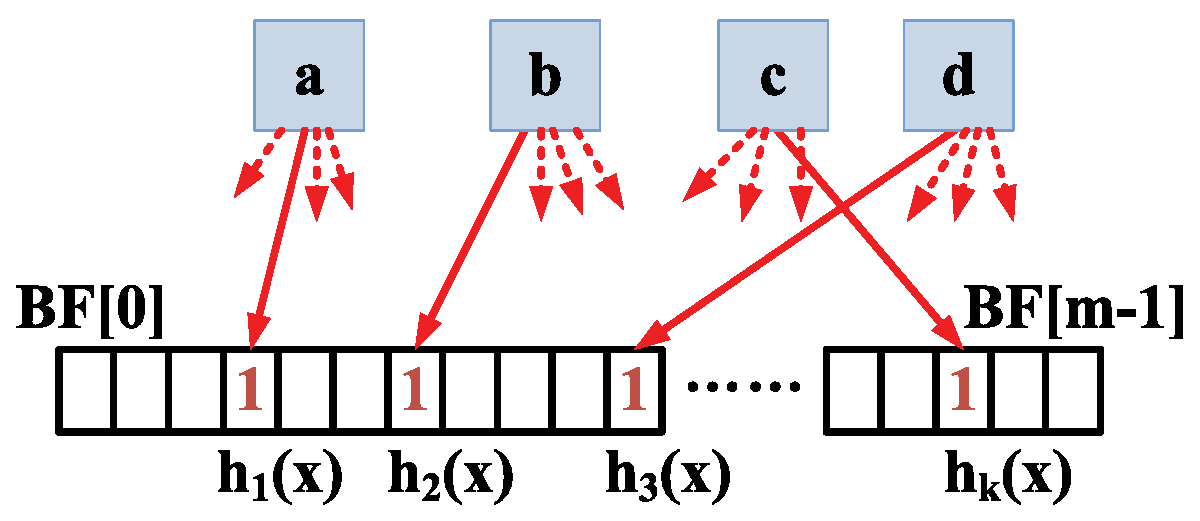
\includegraphics[width=1.4 in]{fig/BFfalse}\label{fig:BFfalse}}
\caption{Basic concept of Bloom filter.}
\label{fig:Operations on basic bloom filter}
\end{figure}

As a probabilistic data structure, the Bloom-filter query may yield a false positive, i.e., the hashing results indicate that the element is in a data set while it actually does not. Suppose $x$ in Fig.\ref{fig:BFfalse} is not in the set, but elements $a, b, c, d$ in the set have already set the corresponding bits to 1. Thus a false positive occurs. After $n$ elements are hashed into Bloom filter, the probability that a specific bit is still 0 can be expressed as: $p = {\left( {1 - \frac{1}{m}} \right)^{kn}} \approx {e^{ - kn/m}}$. The false positive rate of a basic Bloom filter can be computed as
\begin{equation}
%\small
\footnotesize
f = {\left( {1 - p} \right)^k} = {\left( {1 - {e^{ - kn/m}}} \right)^k}.
\label{eq:false positive}
\end{equation}

%In a practical system, we can control the false positive rate to be at a low level by properly setting $m$ and $k$ values for a given $n$ corresponding to the size of the application set.
\subsection{Scalability requirement for big data}
\label{subsec:Scalable bloom filter design for dynamic MCCS}
From (\ref{eq:false positive}), it is easy to observe that the false positive rate increases when $n$ increases.
For a given false positive rate required, $f_0$, the maximum number of elements that a Basic Bloom filter with length $m$ can support is
\begin{equation}
%\small
\footnotesize
{n_0} =  - \left( {\ln \left( {1 - {e^{\ln {f_0}/k}}} \right) \cdot m} \right)/k.
\label{eq:n_0 calculation}
\end{equation}
We call ${n_0}$ the capacity of the Basic Bloom filter with the length $m$ and $k$ hash functions.

Although a basic Bloom filter can work well to represent a static set whose size is known before the design and deployment, it may lead to a high false positive rate with dynamic data arrivals. When the number of data items represented by a BF $n > n_0$, the false rate would be larger than $f_0$, and even approach 1. This would make every new coming data falsely reported to be in the set while it is not, which could render the BF useless. Simply setting $m$ to a large value would help to accommodate more data, but it would lead to high storage and communication overhead  as Bloom filters are usually applied as messages to exchange among distributed nodes in a network.

In addition, without the prior knowledge of the size of the data set, it is also difficult to properly determine the value of $m$.
%but it will introduce high communication cost to maintain the consistency in BF information between cloudlets and mobile users, as a cloudlet needs to piggy-back a long BF vector with its beacons sent periodically.
Instead of designing BF with a static vector length, it would be more efficient to set a proper BF size initially and scale the Bloom filter when the number of data items increases beyond a preset capacity.

\subsection{Design goal}
To control the false positive rate at low level in the presence of varying data set and data arriving speed,  we aim to develop a scalable and flexible bloom filter (SFBF) to support the following three operations:
\begin{itemize}
  \item insert (item $a$): insert item $a$ into the SFBF
  \item extend: extend the SFBF when the size of data set expands beyond the capacity of the current SFBF
  \item query (item $a$): query whether item $a$ is in the data set or not
\end{itemize}

Instead of providing a static expanding solution to handle the scalability problem, the BF design should take flexible and dynamic expanding rate into consideration in the presence of  dynamic set changes in network and distributed systems.



%Although there are various extensions to the basic Bloom filter \cite{tarkoma2012theory},
%they cannot be readily applied in the \rev{big data environment} to solve the scalability problem.
% along with the requirement of application arriving rate aware.
%application's time-dependent weight query.
%In the following subsection, we present our novel scalable and rate-dependent bloom filter.

\section{Design overview}
\label{sec:Scalable and rate-dependent bloom filter}
We design a Scalable and Flexible Bloom filter (SFBF) to control the false positive rate at a low level even when the data items arrive un-predictedly.

As shown in Fig.\ref{fig:Scalable bloom filter design for dynamic MCC}, instead of using a single BF, we consider the use of a BF set consisting of a number of BF vectors to build the SFBF. Originally, SFBF has only one Bloom filter vector, which we call the baseline Bloom filter vector and is denoted as $SFBF_0$. When the data set becomes large with its size exceeding the capacity of the baseline bloom filter, a new bloom filter vector is added to represent the newly arrival elements. The process will continue and more Bloom filter vectors will be added  upon need  for dynamically representing the expanding data set.

\begin{figure}[!h]
\centering
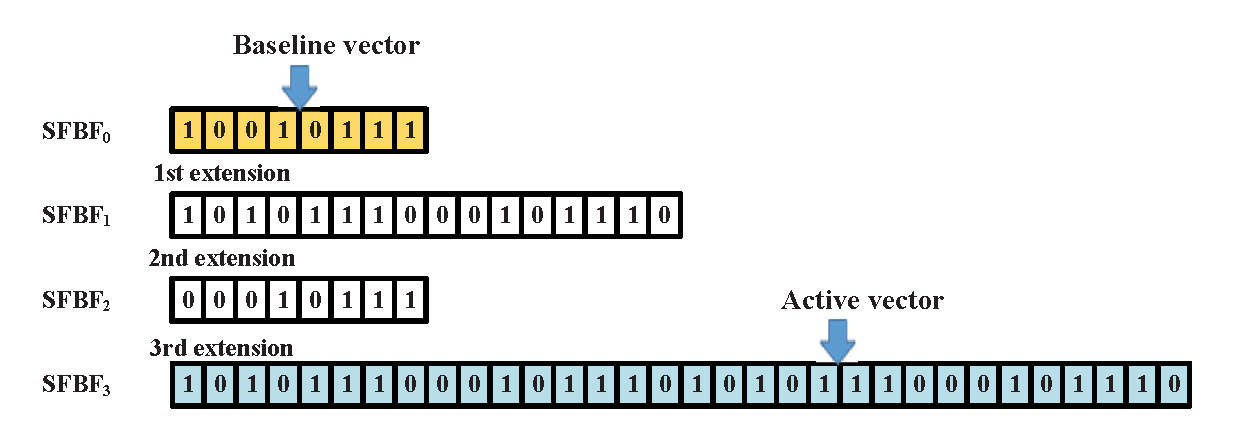
\includegraphics[width=3.0in]{fig/sbf}
\caption{ Scalable and Flexible Bloom filter design for dynamic data set.}
\label{fig:Scalable bloom filter design for dynamic MCC}
\end{figure}
For a SFBF which has expanded $i$ times thus consisting of $i+1$ BF vectors, according to the adding sequence of each BF vector, the vectors can be denoted as $SFBF_0$, $SFBF_1$, $\cdots$, $SFBF_i$.
Among all the BF vectors,  the last added one (i.e., $SFBF_i$) is called the active Bloom filter which is applied to represent the newly arrival data items. We  utilize $n_l$ to record and track the number of items having been represented by the active Bloom filter vector $SFBF_i$.% and $\theta$ can be utilized to identify whether a new extension is needed or not.

The length of the baseline Bloom filter vector is called the baseline length of SFBF, denoted as $m_0$. According to (\ref{eq:n_0 calculation}), given the tolerable false positive rate $f_0$, baseline length $m_0$, and the number of hash functions $k$, the capacity of the baseline BF vector can be calculated as ${n_0} =  - \left( {\ln \left( {1 - {e^{\ln {f_0}/k}}} \right) \cdot m} \right)/k$.

From (\ref{eq:false positive}), we observe that a BF vector's false positive rate $f = {\left( {1 - {e^{ - kn/m}}} \right)^k}$ depends on the number of hash functions $k$ and $\frac{n}{m}$. In our construction process, to ensure the query performance of different vectors to have the same tolerable false positive rate $f_0$, we follow an \emph{\textbf{expanding principle}}. Specifically, we use the same number of hash functions $k$ for each added BF vector, and our expanding will keep the $\frac{{{n_j}}}{{{m_j}}}$ of every BF vector $SFBF_j$ to be the same ($0 \le j \le i$). More especially, the capacity $n_j$ expands proportionally to the length $m_j$ of the added BF vector to keep $\frac{n_j}{m_j}$ the same, i.e., $\frac{{{n_j}}}{{{m_j}}} = \frac{{{n_0}}}{{{m_0}}}$.





Generally, a long BF vector can support more data items at the cost of larger space, while a short BF vector may result in frequent BF expansion. Different from DBF \cite{guo2006theory, wei2010mad2} which adds a fixed-size BF vector each time as the set size increases,  our SFBF adds BF vector with the vector length  determined by the expanding speed. In order to better trade off between the BF extension cost and the space needed, the expanding speed in our paper varies according to practical application requirements.



\begin{algorithm}[h]
\caption{Insertion and Extension Operations}
\label{alg:Insertion Operations}
\begin{algorithmic}[1]
\small
\REQUIRE
SFBF: An SFBF which extends $i$ times with $i+1$ Bloom filter vectors $SFBF_0$, $SFBF_1$, $\cdots$, $SFBF_i$;\\
$a$: A newly arrival data item; \\
$\lambda_{i+1}$: The expanding speed for the  $(i+1)$-th extension;\\
$SFBF_i$: the active Bloom filter vector with its capacity $n_i$;\\
$n_l$: The No. data items represented by the active vector $SFBF_i$


\ENSURE
The update SFBF.\\

\IF{$n_l  = {n_i}$}
\STATE{Add $SFBF_{i+1}$ with ${m_{i+1}} = {2^{{\lambda_{i+1}}-1}} \cdot {m_0}$ }
\STATE{${n_{i + 1}} = {2^{{\lambda_{i+1} } - 1}} \cdot {n_0}$}
\STATE{$i = i+1$}
\STATE{$n_l = 0$}
\ENDIF
\FOR{$1 \le j \le k$}
\STATE{$SFBF_i[{h_j}(a)] = 1$}
\ENDFOR
\STATE{$n_l = n_l+1$}
\end{algorithmic}
\end{algorithm}

Algorithm \ref{alg:Insertion Operations} shows detailed data item insertion and extension  operations for SFBF. For each data insertion, we should first identify whether the SFBF needs an extension or not. If the SFBF needs an extension, a new Bloom filter vector is added and set as the active Bloom filter. All newly arrival data will be inserted and represented by the active Bloom filter vector.

As shown in line 1, if the number of data items represented by the active Bloom filter vector (i.e., $n_l$) reaches its capacity (i.e., ${n_i}$), the SFBF needs a extension. Given the expanding speed for the $(i+1)$-th extension (i.e., ${\lambda _{i+1}}$ ), a new bloom filter vector $SFBF_{i+1}$ with the length ${m_{i+1}} = {m_0}{2^{{\lambda_{i+1}}-1}}$ is added. Note that the length of each newly added Bloom filter is ${2^{\left( {{\lambda _{i+1}} - 1} \right)}}$ times of the baseline length. In Section \ref{sec: Low Cost Information Query and Data Maintenance}, we will utilize this  good properties of BF vector length  to design the hash functions for SFBF and the fast SFBF query algorithm.

According to the expanding principle, to make $\frac{{{m_{i + 1}}}}{{{n_{i + 1}}}} = \frac{{{m_0}}}{{{n_0}}}$,  as shown on line 3, the capacity of the newly added Bloom filter vector is ${n_{i + 1}} = {2^{{\lambda_{i+1} } - 1}} \cdot {n_0}$. Then as shown  on line 4, the newly added Bloom filter vector is set as active Bloom filter vector. A newly arriving data item is inserted to SFBF by setting the corresponding $k$ locations of the active bloom filter vector to 1. Future data items will be hashed to the newest SFBF vector, until  the number of new arriving data items exceeds its capacity and a new SFBF vector is added.




%\begin{algorithm}[h]
%\caption{Insertion and Extension Operations}
%\label{alg:Insertion and Extension Operations}
%\begin{algorithmic}[1]
%\textbf{Initiation Operation}
%\STATE{Initiate the Bloom filter's basic parameters: length $m_0$, $k$ hash functions, the reference arrival rate $r_0$, the required false positive rate $f_0$.}
%\STATE{Initiate an SFBF vector $SFBF_0$ with these basic parameters. Let $n_0$ denote the maximum number of data items to keep $SFBF_0$'s false positive rate satisfying $f \le f_0$, initiate $n_0$ by applying $m=m_0$ to (\ref{eq:n_0 calculation}).}
%\STATE{Let $i$ denote the last SFBF vector. Initiate $i=0$. Let $n_i$ denote the maximum number of data items to keep current $SFBF_i$'s false positive rate satisfying $f \le f_0$ with $SFBF_i$'s length $m_i$.}
%\STATE{Let $C$ denote the total number of data items represented by the last SFBF vector, initiate $C=0$.}
%\textbf{\\Insertion Operation (when a data item $a$ arrives).}
%\IF{$C=n_i$}
%\STATE{SFBF needs an extension, and $i=i+1$. Let $d_T$ denote duration from the time of last SFBF extension to the current time, calculate the data arriving rate $r(i-1)=C/d_T$.}
%\STATE{A new SFBF vector $SFBF_i$ is added to SFBF with the vector length ${m_i} = {2^{\left\lceil {r(i-1)/{r_0}} \right\rceil -1 }} \cdot {m_0}$, calculate ${n_i} = {2^{\left\lceil {r(i-1)/{r_0}} \right\rceil -1 }} \cdot {n_0}$, update hash functions with their hash range from $m_{i-1}$ to $m_i$, and reset $C=0$.}
%\ENDIF
%\STATE{Insert the data item $a$ to the last $SFBF_i$ by setting the corresponding bit to 1, that is, $SFBF[{h_j}(a)] = 1$, for $1 \le j \le k$, update $C=C+1$.}
%\end{algorithmic}
%\end{algorithm}
\begin{figure}[!h]
\centering
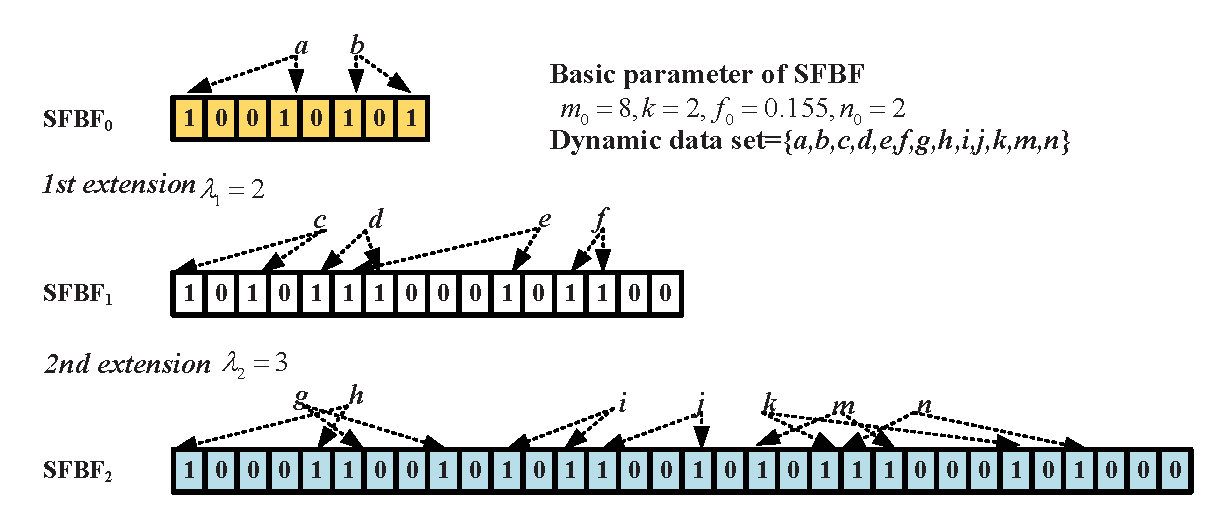
\includegraphics[width=3.0in]{fig/SFBFexample}
\caption{Example of SFBF.}
\label{fig:Example of SFBF.}
\end{figure}

Fig.\ref{fig:Example of SFBF.} illustrates how an SFBF works. The SFBF is utilized to represent a dynamic data set with sequentially arriving data items  $a, b, c, d, e, f, g, h, i, j, k, m, n$. The baseline Bloom filter vector is $SFBF_0$ with  the length $m_0=8$ and the number of hash functions $k=2$. For a better explanation, we assign a big false positive rate $f_0=0.155$ for this Bloom filter, and the Bloom filter can support $n_0=2$ data items according to (\ref{eq:n_0 calculation}).

When the data item $c$ arrives, two data items $a$ and $b$ have been represented by $SFBF_0$, and $n_l=n_0=2$. According to the line 1 of Algorithm \ref{alg:Insertion Operations}, a new SFBF vector should be added. Given the expanding speed ${\lambda _1} = 2$, according to the line 2 of Algorithm \ref{alg:Insertion Operations}, we can create a double-size new $SFBF_1$ of 16 bits to represent the new data item $c$.

When the data item $g$ arrives, SFBF needs an extension again because $SFBF_1$ has already represented data items $c, d, e, f$, and the number of data items represented $n_l$ is equal to $SFBF_1$'s capacity $n_1=4$.
%\note{You $n_1$ should be 2 or 4? You also have a $n_0$, right? The total offloaded should be the sum of these two. Dear sister, $n_1=4$. $C$ denote the number of applications represented by the last Bloom filter vector}
Given the expanding speed ${\lambda _2} = 3$,  a new $SFBF_2$ of 32 bits is created to represent the new data items. Therefore, all the data items $a, b, c, d, e, f, g, h, i, j, k, m, n$ can be represented in SFBF by an array of BF vectors $SFBF_0$, $SFBF_1$, and $SFBF_2$ with only two extensions.

\section{Challenge of SFBF}
\label{sec:Challenge in SFBF}
To make the Bloom filter scalable with the size of the data set, the key technique taken by SFBF is to add a new BF vector upon need. The length of the BF vector is determined by the expanding speed instead of being fixed.
  As a result, SFBF usually consists of multiple BF vectors with various lengths. %which makes the design of quick Bloom filter query algorithm very difficult.


%\subsection{Hash function design requirement for SFBF}
%\label{subsec:Hash function design requirement for SFBF}
Conventionally, a group of hash functions are preset to support a BF vector, and the value of each hash function will fall within the length range of the BF. As an array of BF vectors are used in SFBF with the length of each vector determined by the expanding speed, each BF vector needs its own group of hash functions according to its length.

In the example of Fig.\ref{fig:Example of SFBF.}, three BF vectors $SFBF_0$, $SFBF_1$, and $SFBF_2$ are created with the vector lengths $m_0$, $2m_0$, and $4m_0$, respectively. Thus, three groups of hash functions need to be generated, with each having $k$ hash functions. The hash range of each group should match the length of the corresponding BF vector, as shown in Fig.\ref{fig:Hash range requirement.}.

\begin{figure}[!h]
\centering
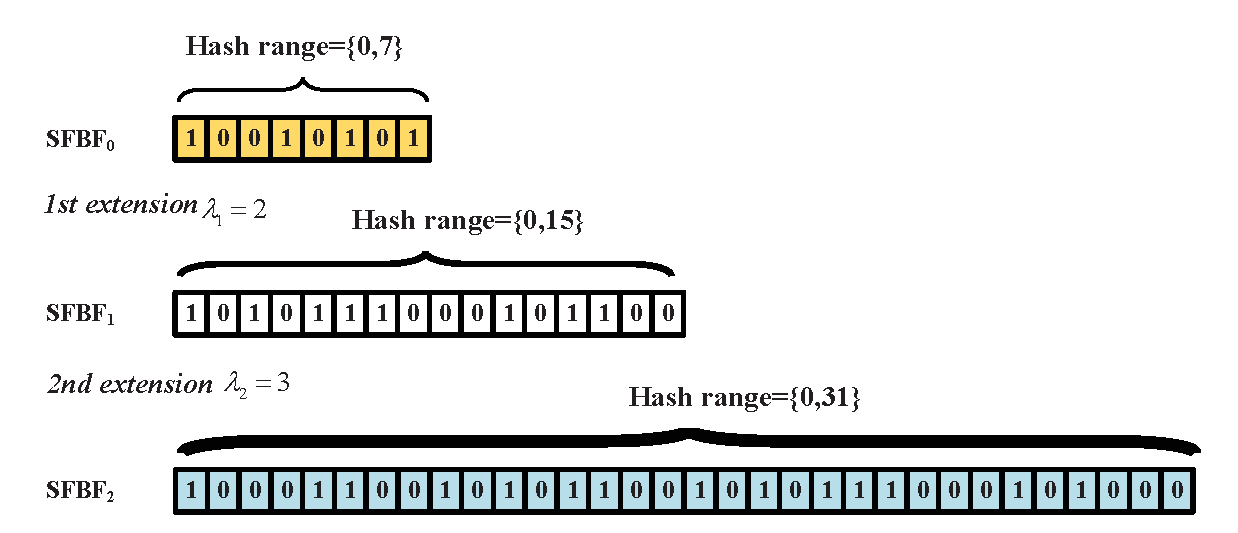
\includegraphics[width=3.0in]{fig/HashRange}
\caption{Hash range requirement.}
\label{fig:Hash range requirement.}
\end{figure}

If SFBF is applied to determine whether an element  is  a member of the data set, all the BF vectors should be tested in the worst case which would involve $(i+1) \times k$ hash computation. Although one group of hash functions can be applied to the same-length Bloom filter vectors, as SFBF consists of multiple BF vectors with various lengths, the query algorithm will involve a lot of hash computations. The high computational cost is the main challenge in realizing SFBF.



%To obtain the hash functions needed for each SFBF vector, a cloudlet can generate a new group hash functions when a new SFBF vector needs to be added and announce these hash functions to mobile users. Alternatively, different groups of hash functions may be stored on a cloudlet and close-by mobile devices in advance. However, transferring and storing multiple groups of hash functions in resource limited wireless system would introduce high communication and/or storage cost. In addition, without knowing the SFBF vector length and the number of applications to offload in advance, it is difficult to determine the hash functions to use and how many groups of hash functions would be needed.

To simplify the hash function generation procedure and more importantly to ensure light-weight query and low-cost maintenance of  SFBF, we propose an algorithm to adaptively generate hash functions according to the length of BF vector  in Section \ref{sec:Adaptive Hash function Generation}, based on which, we further propose a fast BF query algorithm in Section \ref{sec: Low Cost Information Query and Data Maintenance}.

% In next, section, before we present our adaptive hash function generation algorithm, we first review $h_3$ hash function in next subsection.



%Although the proposed offloading management mechanism is promising and the operations are simple, the basic Bloom filter cannot be directly applied in dynamic MCCS. In this section, we first analyze the problems, and then present our design of rate-dependent Bloom filter.

%\subsection{Construction of Rate-dependent Bloom Filter}
%\label{sec:Construction of Rate-dependent Bloom Filter}






%We construct SFBF depending on the application arrival rate, as
%shown
%Algorithm \ref{alg:Basic Operations of Rate-dependent Bloom filter} illustrates the construction process of SFBF. We denote the initial reference data arriving rate as $r_0$, and the initial Bloom filter length $m_0$. At a given time, suppose $i-1$ SFBF vectors have been added, i.e., SFBF has vectors 0, 1, ..., $i$-1. If the existing number of data items have reached the limit that the current sequence of SFBF vectors can hold, a new SFBF vector will be added. Denote the data arriving rate estimated during the previous SFBF interval as $r(i-1)$, then the length of SFBF vector to add in the $i$th extension is set to ${m_i} = {2^{\left\lceil {r(i-1)/{r_0}} \right\rceil -1 }} \cdot {m_0}$, and the number of data items supported by the newly added SFBF vector is calculated as ${n_i} = {2^{\left\lceil {r(i-1)/{r_0}} \right\rceil -1 }} \cdot {n_0}$. Let $C$ denote the total number of data items represented by the last SFBF vector and $d_T$ denote the duration from the time instant of the last SFBF extension to the current time, the data arriving rate can be simply estimated as $r(i-1)=C/d_T$. Accordingly hash functions will be updated with the hash range set to be from $m_{i-1}$ to $m_i$. Future data items will be hashed to the newest SFBF vector, until a new SFBF vector is added when the number of new arriving data items exceeds  ${n_i}$.
%
%Long BF vector can support more data items at the cost of larger space, while short BF vector may result in frequent BF expansion. In order to better trade off between the BF extension cost and the space needed, we apply the arriving rate $r(i-1)$ as a reference to determine the length $m_i$ of the new SFBF vector, where ${m_i} = {2^{\left\lceil {r(i-1)/{r_0}} \right\rceil -1 }} \cdot {m_0}$.
%
%%Moreover, in the SFBF design,
%From (\ref{eq:false positive}), we observe that a BF vector's false positive rate $f = {\left( {1 - {e^{ - kn/m}}} \right)^k}$ depends on the number of hash functions $k$ and $\frac{n}{m}$. In our construction process, to ensure the query performance of different vectors to have the same maximum tolerable false positive rate $f_0$, we take an \emph{\textbf{expanding principle}}. Specifically,  we use the same number of hash functions $k$ for each added BF vector, and our expanding will keep the $\frac{{{n_i}}}{{{m_i}}}$ of every BF vector $SFBF_i$ to be the same. More especially, the capacity $n_i$ expands proportionally to the length $m_i$ of the added BF vector to keep $\frac{n_i}{m_i}$ the same, i.e., $\frac{{{n_i}}}{{{m_i}}}=\frac{{{2^{\left\lceil {r\left( {i - 1} \right)/{r_0}} \right\rceil  - 1}} \cdot {n_0}}}{{{2^{\left\lceil {r\left( {i - 1} \right)/{r_0}} \right\rceil  - 1}} \cdot {m_0}}} = \frac{{{n_0}}}{{{m_0}}}$.
%
%
%The reference rate $r_0$ has a direct impact on the SFBF's expanding speed and the length of BF vector newly extended. An optimal $r_0$ depends on the statistics of data arriving speed and may change adaptively with time. How to set optimal $r_0$ is out of this paper's focus. In this paper, $r_0$ is initialized based on the data arriving speed $r(0)$ before the first extension, and we set $r_0=r(0)$.
%\note{How could you know this if it is not simulation? Dear sister, in this paper, we just set $r_0=r(0)$.  No one knows what $r(0)$ is.Dear sister, $r(0)$ can be calculated when the first BF expanding needed.)}

%\subsection{An Example SFBF}
%The basic idea of SFBF can be illustrated through an example.


\section{Adaptive hash function generation}
\label{sec:Adaptive Hash function Generation}
In this section,
%we first discuss the challenge and requirement on the design of hash functions used in SFBF. We then
we first  introduce the basic $H_3$ hash function, and then propose a new adaptive hash function generation algorithm.


\subsection{Review of $H_3$ hash function}
\label{subsec:The review of $H_3$ hash function}
$H_3$ hash function is a universal class of hash function introduced by Carter and Wegman \cite{carter1979universal}.
%In order to increase randomness with a low probability for the hashed values of a pair of input keys to collide, $H_3$ hash functions are also applied in Bloom filters ~\cite{ramakrishna1989practical,kocak2006low}.
 Requiring only Boolean AND and XOR operations to calculate the key's hash value, $H_3$ hash functions are easy to implement using either software or hardware ~\cite{ramakrishna1997efficient,ramakrishna1991perfect}.

Each hash function in $H_3$ class is a linear transformation ${B^T} = {Q_{r \times w}}{A^T}$ that maps a $w$-bit binary string $A = {a_1}{a_2} \cdots {a_w}$ to an $r$-bit binary string $B = {b_1}{b_2} \cdots {b_r}$ as follows:

\begin{equation}
%\small
\footnotesize
\left( {\begin{array}{*{20}{c}}
   {{b_1}}  \\
   {{b_2}}  \\
    \vdots   \\
   {{b_r}}  \\
\end{array}} \right) = \left( {\begin{array}{*{20}{c}}
   {{q_{11}}} & {{q_{12}}} &  \cdots  & {{q_{1w}}}  \\
   {{q_{21}}} & {{q_{22}}} &  \cdots  & {{q_{2w}}}  \\
    \cdots  &  \cdots  &  \cdots  &  \cdots   \\
   {{q_{r1}}} & {{q_{r2}}} &  \cdots  & {{q_{rw}}}  \\
\end{array}} \right)\left( {\begin{array}{*{20}{c}}
   {{a_1}}  \\
   {{a_2}}  \\
    \vdots   \\
   {{a_w}}  \\
\end{array}} \right)
\label{eq:h3hash}
\end{equation}

\noindent where $A$ and $B$ are the input key (index) and its hash value, and the hash generation matrix ${Q_{r \times w}}$ is an $r \times w$ matrix defined over $GF(2)=\{0,1\}$ with each $H_3$ hash function uniquely corresponding to such a ${Q_{r \times w}}$. The hash function of ${Q_{r \times w}}$ can map the key ranged in $\{0,{2^w} - 1\}$ to a hash value ranged in $\{0,{2^r} - 1\}$.

The multiplication and addition in $GF(2)$ is Boolean AND($\bullet$) and XOR($\oplus$), respectively. According to (\ref{eq:h3hash}), each bit of $B$ is calculated as follows:
\begin{equation}
%\small
\footnotesize
{b_i} = \left( {{a_1} \bullet {q_{i1}}} \right) \oplus \left( {{a_2} \bullet {q_{i2}}} \right) \oplus  \cdots  \oplus \left( {{a_w} \bullet {q_{iw}}} \right){\rm{   }}\left( {i = 1,2, \cdots ,r} \right)
\label{eq:h3hashbit}
\end{equation}
%If we use column vector ${d_j}\left( {1 \le j \le w} \right)$ to denote the hash generation matrix ${Q_{r \times w}}$, then matrix ${Q_{r \times w}} = \left( {\begin{array}{*{20}{c}}
%   {{d_1},} & {{d_2},} &  \cdots  & {,{d_w}}  \\
%\end{array}} \right)$ . A multiplication AND($\bullet$) of a bit and a vector ${a_j} \bullet {d_j}$ can be defined as follows:
%\begin{equation}
%%\small
%\footnotesize
%{a_j} \bullet {d_j} = {a_j} \bullet \left( {\begin{array}{*{20}{c}}
%   {{q_{1j}}}  \\
%   {{q_{2j}}}  \\
%    \vdots   \\
%   {{q_{rj}}}  \\
%\end{array}} \right) = \left( {\begin{array}{*{20}{c}}
%   {{a_j}}  \\
%   {{a_j}}  \\
%    \vdots   \\
%   {{a_j}}  \\
%\end{array}} \right) \bullet \left( {\begin{array}{*{20}{c}}
%   {{q_{1j}}}  \\
%   {{q_{2j}}}  \\
%    \vdots   \\
%   {{q_{rj}}}  \\
%\end{array}} \right) = \left( {\begin{array}{*{20}{c}}
%   {{a_j} \bullet {q_{1j}}}  \\
%   {{a_j} \bullet {q_{2j}}}  \\
%    \vdots   \\
%   {{a_j} \bullet {q_{rj}}}  \\
%\end{array}} \right)
%\label{eq:h3hashbit}
%\end{equation}
%Then, the r-bit binary string can be expressed in a straight way:
%\begin{equation}
%%\small
%\footnotesize
%{B^T} = h(A) = \left( {{a_1} \bullet {d_1}} \right) \oplus \left( {{a_2} \bullet {d_2}} \right) \oplus  \cdots  \oplus \left( {{a_w} \bullet {d_w}} \right)
%\label{eq:h3hashbit}
%\end{equation}

We take two examples to illustrate the $H_3$ class hash function. In the first example, the hash generation matrix is
\begin{equation}
%\small
\footnotesize
{Q_{2 \times 8}} = \left( {\begin{array}{*{20}{c}}
   0 & 1 & 1 & 0 & 1 & 1 & 0 & 1  \\
   1 & 1 & 0 & 0 & 0 & 1 & 0 & 0  \\
\end{array}} \right),
\label{eq:h1matrix}
\end{equation}
where $w=8$, $r=2$, and the hash function is used to map the input key (index) to its hash value: $\left\{ {0, \ldots ,{{\rm{2}}^{\rm{8}}} - {\rm{1}} = {\rm{255}}} \right\} \to \left\{ {0, \ldots ,{{\rm{2}}^{\rm{2}}} - {\rm{1}} = {\rm{3}}} \right\}$. Under this hash function, the hash value for index 69 can be calculated by Eq.(\ref{eq:h3hash}), expressed as follows
\begin{equation}
%\small
%\footnotesize
\scriptsize
\begin{array}{l}
 h_1\left( {69} \right) = h_1\left( {{\rm{01000101}}} \right) \\
  = \left( {\begin{array}{*{20}{c}}
   0 & 1 & 1 & 0 & 1 & 1 & 0 & 1  \\
   1 & 1 & 0 & 0 & 0 & 1 & 0 & 0  \\
\end{array}} \right)\left( {\begin{array}{*{20}{c}}
   0  \\
   1  \\
   0  \\
   0  \\
   0  \\
   1  \\
   0  \\
   1  \\
\end{array}} \right) = \left( {\begin{array}{*{20}{c}}
   1  \\
   0  \\
\end{array}} \right) \\
 \end{array}
\label{eq:h3example1}
\end{equation}
where ${\left( {\begin{array}{*{20}{c}}
   1  \\
   0  \\
\end{array}} \right)^T} = \left( {\begin{array}{*{20}{c}}
   1 & 0  \\
\end{array}} \right) = 2\left( {decimal} \right)$, so the hash value of 69 under the hash function $h_1$ is $h_1(69)=2$.

In the second example, the hash generation matrix is
\begin{equation}
%\small
\footnotesize
{Q_{3 \times 8}} = \left( {\begin{array}{*{20}{c}}
   0 & 1 & 1 & 0 & 1 & 1 & 0 & 1  \\
   1 & 1 & 0 & 0 & 0 & 1 & 0 & 0  \\
   0 & 0 & 0 & 1 & 1 & 1 & 1 & 0  \\
\end{array}} \right),
\label{eq:h2matrix}
\end{equation}
where $w=8$ and $r=3$. Similarly, the hash value for index 69 can be calculated as follows

\begin{equation}
%\small
%\footnotesize
\scriptsize
\begin{array}{l}
 {h_2}\left( {69} \right) = h_2\left( {{\rm{01000101}}} \right) \\
  = \left( {\begin{array}{*{20}{c}}
   0 & 1 & 1 & 0 & 1 & 1 & 0 & 1  \\
   1 & 1 & 0 & 0 & 0 & 1 & 0 & 0  \\
   0 & 0 & 0 & 1 & 1 & 1 & 1 & 0  \\
\end{array}} \right)\left( {\begin{array}{*{20}{c}}
   0  \\
   1  \\
   0  \\
   0  \\
   0  \\
   1  \\
   0  \\
   1  \\
\end{array}} \right) = \left( {\begin{array}{*{20}{c}}
   1  \\
   0  \\
   1  \\
\end{array}} \right) \\
 \end{array}
\label{eq:h3example2}
\end{equation}
\noindent and ${\left( {\begin{array}{*{20}{c}}
   1  \\
   0 \\
   1  \\
\end{array}} \right)^T} = \left( {\begin{array}{*{20}{c}}
   1 & 0 & 1  \\
\end{array}} \right) = 5\left( decimal \right)$, then the hash value of 69 under the hash function $h_2$ is $h_2(69)=5$.

In these two examples, the same input index 69 is hashed to different values using two different hash functions. When comparing the matrices in Eq.(\ref{eq:h2matrix}) and Eq.(\ref{eq:h1matrix}), we observe that the matrix in Eq.(\ref{eq:h2matrix}) has one more row and their first two rows are the same. In~Section \ref{sec: Low Cost Information Query and Data Maintenance}, we will investigate the relationship of these
similar matrices and exploit the hash matrix features to design a light weight query algorithm for SFBF.

\subsection{Hash function generation}
From the basic structure of a $H_3$ hash function, the hash value range is determined by the number of rows of its hash generation matrix. Therefore, we can generate different value-range hash functions using one base matrix, with the number of rows to select from the base matrix adapted according to the length of the BF vector.  In order to generate $k$ hash functions for each SFBF vector, we only need one group of  $k$ base generation matrices ${Q_{R \times w}}[1],{Q_{R \times w}}[2], \cdots ,{Q_{R \times w}}[k]$.

In order to reduce the overhead for hash function generation and speed up BF query, we propose to generate hash functions for different SFBF vectors from the same $k$ base matrices, ${Q_{R \times w}}[1],{Q_{R \times w}}[2], \cdots ,{Q_{R \times w}}[k]$. The generation process is presented in Algorithm \ref{alg:Adaptive hash function generation}. For a given $SFBF_i$ whose length is $m_i$, the hash functions are generated by selecting the first $l_i$ rows of ${Q_{R \times w}}$ of the base generation matrices, where $l_i$ is determined by $l_i = {\log _2}{m_i}$.








\begin{algorithm}[h]
\caption{Adaptive hash function generation}
\label{alg:Adaptive hash function generation}
\begin{algorithmic}[1]
\small
%\footnotesize
\REQUIRE
$k$ base hash generation matrices ${Q_{R \times w}}[1]$,${Q_{R \times w}}[2]$, $\cdots$,${Q_{R \times w}}[k]$. \\
A vector $SFBF_i$ with its length $m_i$.\\
\ENSURE
$k$ hash functions for $SFBF_i$.\\

\STATE{Calculate the number of rows $l_i$ needed to form the hash generation matrix for $SFBF_i$ according to its length: ${l_i} = {\log _2}{m_i}$.}
%following the equation of
%\begin{equation}
%\small
%{l_i} = {\log _2}{m_i}
%\end{equation}
%}
\STATE{Select the first $l_i$ rows of the base hash generation matrices ${Q_{R \times w}}[u], 1 \le u \le k$ to form the hash matrices ${Q_{l_i \times w}}[u], 1 \le u \le k$ for $SFBF_i$.}
\STATE{Return ${Q_{l_i \times w}}[1],{Q_{l_i \times w}}[2], \cdots ,{Q_{l_i \times w}}[k]$.}
\end{algorithmic}
\end{algorithm}

Fig.~\ref{fig:Hash function generated from base matrix} presents an example to illustrate Algorithm \ref{alg:Adaptive hash function generation}. For $SFBF_0$, as $m_0=8$, the first ${\log _2}\left( {{m_0}} \right)=3$ rows in the base matrix are extracted to build the hash function. Similar processes are adopted to generate the hash functions for $SFBF_1$ and $SFBF_2$. As the lengths of $SFBF_1$ and $SFBF_2$ are 16 and 32, the hash functions for $SFBF_1$ and $SFBF_2$ are 4 rows and 5 rows, respectively.  As the hash functions for different BF vectors are generated from the same base matrix, it creates strong relationship among the hash values calculated for different BF vectors. This feature can be exploited to largely reduce the computation cost for BF query, as shown in Section \ref{sec: Low Cost Information Query and Data Maintenance}.


\begin{figure}[!h]
\centering
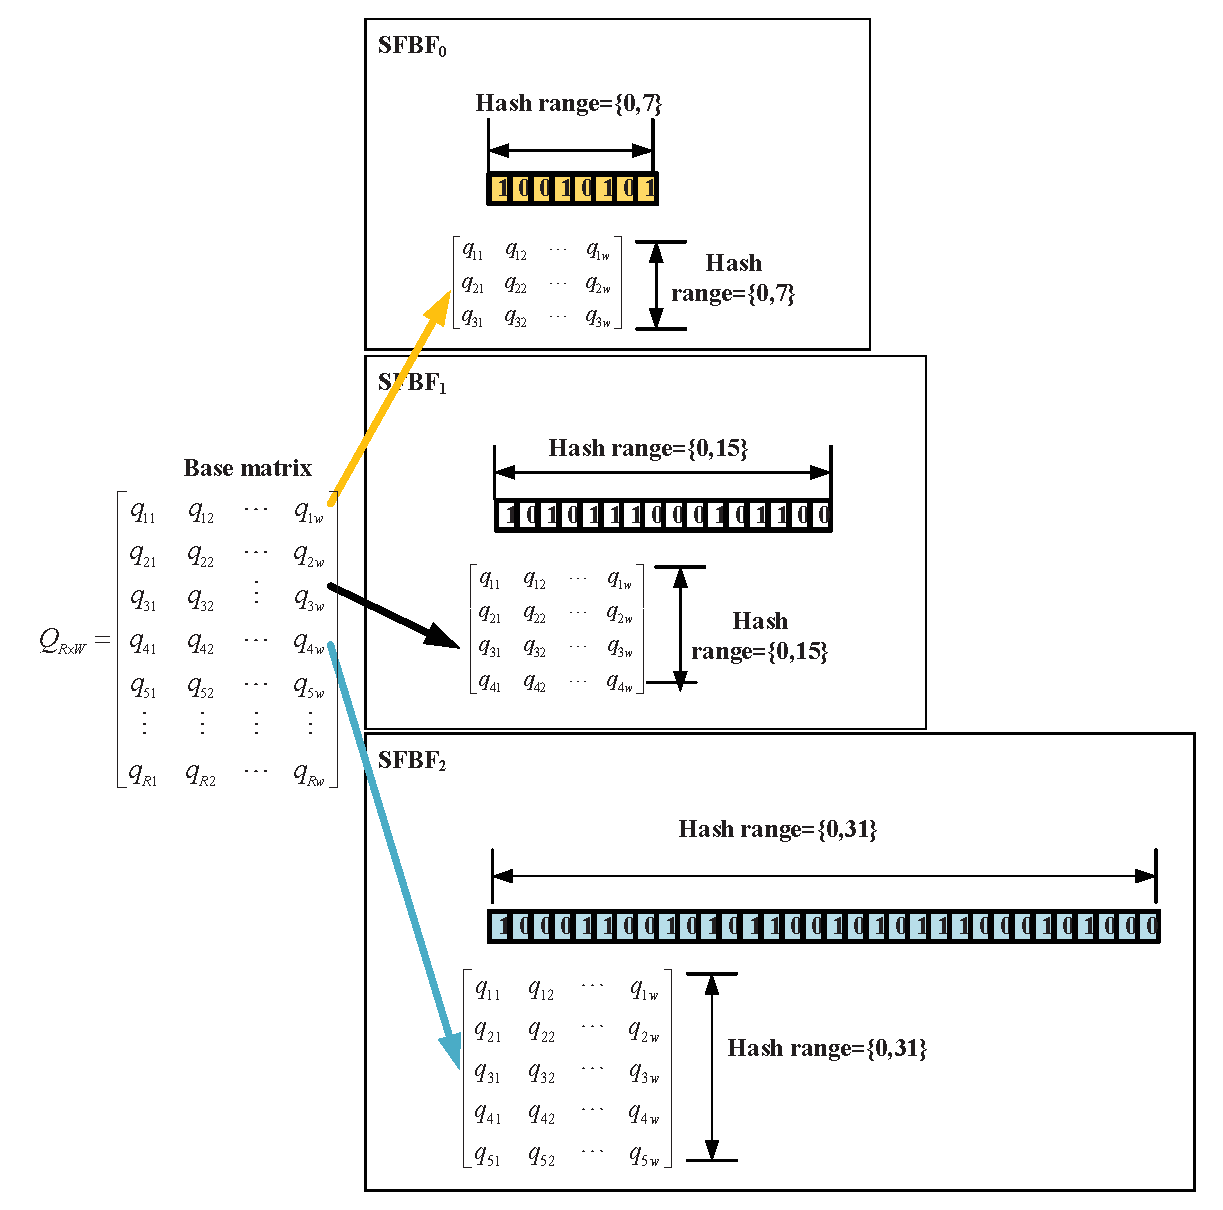
\includegraphics[width=3.0 in]{fig/Hash_function_generated_from_base_matrix}
\caption{Different hash functions for different BF vectors are generated from the same base matrix.}
\label{fig:Hash function generated from base matrix}
\end{figure}

With Algorithm \ref{alg:Adaptive hash function generation}, the SFBF insertion operation in Algorithm \ref{alg:Insertion Operations}
 can be described more clearly as follows.
%At the very beginning, SFBF begins with $SFBF_0$ of the vector length $m_0$. According to Algorithm \ref{alg:Adaptive hash function generation}, we generate $k$ hash functions for $SFBF_0$ with their hash generation matrices consisting of the first $l_0$ rows of the base matrices, where $l_0 = log_2m_0$, denoted as ${Q_{{l_0} \times w}}[u], 1 \le u \le k$. When a new application $q$ is offloaded to the cloudlet and needed to insert into the $SFBF_0$, the hash functions defined by these hash generation matrices ${Q_{{l_0} \times w}}[u]$ are applied to the application $q$ to obtain the $k$ locations ${Q_{{l_0} \times w}}[u](q)$, and set these $k$ bits at $SFBF_0[{Q_{{l_0} \times w}}[u](q)], 1 \le u \le k$ to 1.
During the $i$th extension, a new $SFBF_i$ is added to SFBF with the vector length ${m_i} = {2^{\lambda_i  - 1}} \cdot {m_0}$, where $\lambda_i$ is the  expanding speed. According to Algorithm \ref{alg:Adaptive hash function generation},
the corresponding $k$ hash functions are generated by selecting the first ${l_i} =\log_2m_i= {\log _2}\left( {2^{\lambda_i  - 1}} \cdot {m_0} \right) = \lambda_i  - 1 + {l_0}$ rows of the base matrices where ${l_0} = {\log _2}\left( {{m_0}} \right)$, denoted as ${Q_{{l_i} \times w}}[u], 1 \le u \le k$. All data items to insert into $SFBF_i$ should use these hash functions to find the corresponding bits in $SFBF_i$ and set them to 1.


It is worth pointing out that, although our SFBF consists of multiple SFBF vectors,
we only need to store one group of $k$ base matrices ${Q_{R \times w}}[1],{Q_{R \times w}}[2], \cdots ,{Q_{R \times w}}[k]$ at the very beginning. To support unpredictably high expanding speed and thus the large length of SFBF vector, the number of rows $R$ in these bash matrices are initially set to a large value.
Our generation algorithm is very simple and can support fast BF query as we will see in Section~\ref{sec: Low Cost Information Query and Data Maintenance}.

\section{Low cost SFBF query and maintenance}
\label{sec: Low Cost Information Query and Data Maintenance}
In this section, we first analyze the special requirement for SFBF query, and then investigate the relationship of
hash functions generated by Algorithm \ref{alg:Adaptive hash function generation}. Based on the analysis, we propose a light-weight query algorithm, and present our low-cost SFBF filter maintenance schemes.

\subsection{SFBF query requirement}
For an SFBF vector $SFBF_j$, to determine if a data item $q$ has already been inserted into the vector, it will check whether $SFBF_j[{h_1}\left( {{q}} \right)],SFBF_j[{h_2}\left( {{q}} \right)], \cdots, SFBF_j[{h_k}\left( {{q}} \right)]$ with positions calculated by corresponding $k$ hash functions all set to 1. For an SFBF with the initial BF vector plus $i$ extensions, in the worst case, it needs to search through the whole array of SFBF vectors, and the query procedure would require $k(i+1)$ times of hash computations. This  introduces not only high computation cost but also long searching time.

In this section, we design a light weight query algorithm which can largely reduce the total times of hash computations  from $k(i+1)$ to $k$. Before  presenting our query algorithm, we first analyze the relationship of the generated hash functions.

\subsection{Relationship of generated hash functions}
Among SFBF vectors, we can find the longest vector $SFBF_{max}$ with the length $m_{max}$, and denote ${l_{\max }} = {\log _2}{m_{\max }}$. From our proposed hash generation algorithm, the $k$ hash functions for $SFBF_{max}$ can be obtained by taking the first $l_{max}$ rows of $k$ base matrices respectively, denoted as ${Q_{{l_{\max }} \times w}}[1],{Q_{{l_{\max }} \times w}}[2], \cdots ,{Q_{{l_{\max }} \times w}}[k]$.

Theorem \ref{th:hash address} will show that for a given data item $q$, if we have the hash values for $SFBF_{max}$,
 %under the hash functions ${Q_{{l_{\max }} \times w}}[1],{Q_{{l_{\max }} \times w}}[2], \cdots ,{Q_{{l_{\max }} \times w}}[k]$,
 the corresponding hash values for other SFBF vectors under their corresponding hash functions can be easily deduced by simply right-shifting the hash values calculated for $SFBF_{max}$.

Before presenting the Theorem, we first introduce the bit logic shifting operation using two examples in Fig.\ref{fig:Logic shift operation}. The bit logic shifting is a bitwise operation performing on the binary representation of an integer, where zeros are shifted in to replace the discarded bits. In this paper, we use right logic shift operation ($>>$) to deduce hash values.


\begin{figure}[!h]
\centering
\subfigure[Left logic shift]{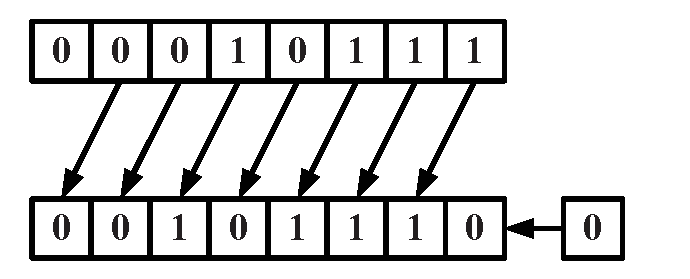
\includegraphics[width=1.4 in]{fig/Left_logical_shift}
\label{fig:Left logic shift}}
\subfigure[Right logic shift]{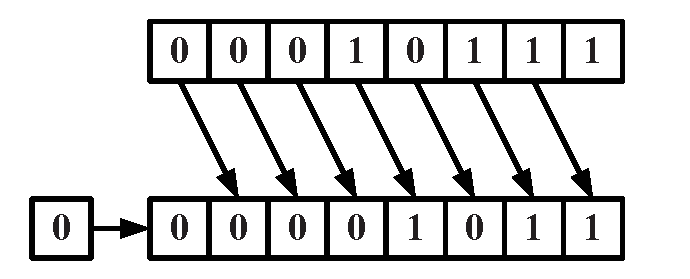
\includegraphics[width=1.4 in]{fig/right_logical_shift}
\label{fig:Right logic shift}}
\caption{Logic shift operation.}
\label{fig:Logic shift operation}
\end{figure}


\newtheorem{theorem}{\textbf{Theorem}}
\begin{theorem}
\label{th:hash address}
Suppose the data item $q$'s hash values under hash functions of ${Q_{{l_{\max }} \times w}}[u]$ where $(1 \le u \le k)$ for BF vector $SFBF_{max}$ are $Add{r_{max}}\left[ u \right]{\rm{ }}(q)$, then
\begin{equation}
\small
%\footnotesize
Add{r_j}\left[ u \right](q) = Add{r_{\max }}\left[ u \right](q) >  > ({\log _2}{m_{\max }} - {\log _2}{m_j})
\label{eq:false whole}
\end{equation}
where $Add{r_j}\left[ u \right](q){\rm{ }}({\rm{1}} \le u \le k)$ are the hash values of the data item $q$ under the hash functions for vector $SFBF_j$ whose length is $m_j$.
\end{theorem}
\begin{proof}
The base generation matrix ${Q_{R \times w}}\left[ u \right]{\rm{ }}({\rm{1}} \le u \le k)$ is
\begin{equation}
%\small
%\footnotesize
\scriptsize
{Q_{R \times w}}[u] = \left[ {\begin{array}{*{20}{c}}
   {{q_{11}}} & {{q_{12}}} &  \cdots  & {{q_{1w}}}  \\
   {{q_{21}}} & {{q_{22}}} &  \cdots  & {{q_{2w}}}  \\
    \vdots  &  \vdots  &  \vdots  &  \vdots   \\
   {{q_{{l_j}1}}} & {{q_{{l_j}2}}} &  \cdots  & {{q_{{l_j}w}}}  \\
    \vdots  &  \vdots  &  \vdots  &  \vdots   \\
   {{q_{{l_{\max }}1}}} & {{q_{{l_{\max }}2}}} &  \cdots  & {{q_{{l_{\max }}w}}}  \\
    \vdots  &  \vdots  &  \vdots  &  \vdots   \\
   {{q_{R1}}} & {{q_{R2}}} &  \cdots  & {{q_{Rw}}}  \\
\end{array}} \right]
\end{equation}
Let ${l_j} = {\log _2}{m_j}$. According to Algorithm \ref{alg:Adaptive hash function generation}, the hash functions for $SFBF_j$ are hash functions with their hash matrices consisting of the first $l_j$ rows of the base generation matrices, that is ${Q_{{l_j} \times w}}\left[ u \right]{\rm{ }}({\rm{1}} \le u \le k)$.

Let the bit string of data item $q$'s index be $x = {a_1}{a_2} \cdots {a_w}$. The bit strings of the two hash values $Add{r_{max}\left[ u \right] (q)}$ and $Add{r_{j}\left[ u \right] (q)}$ are  ${s_1}{s_2} \cdots s_{l_{\max }}$ and ${t_1}{t_2} \cdots t_{l_j}$, respectively.


\begin{figure}[!h]
\centering
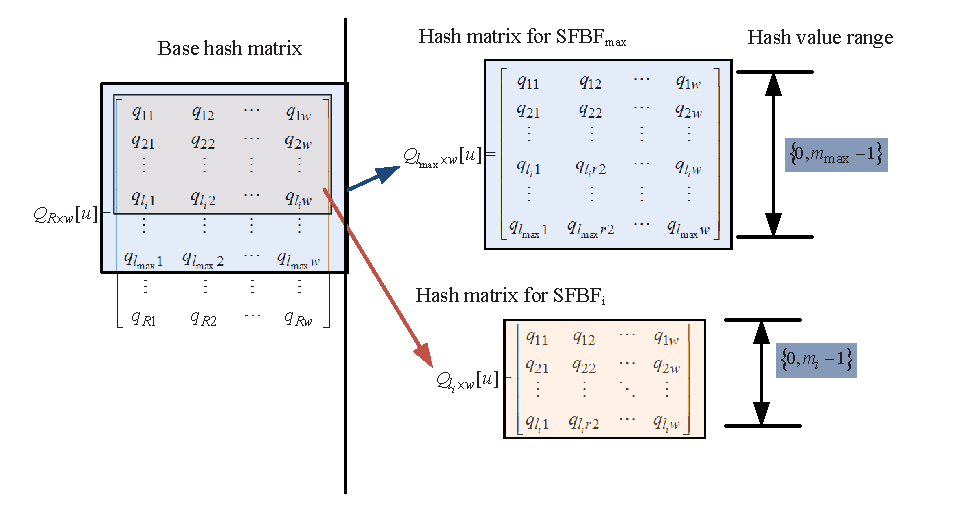
\includegraphics[width=3.2 in]{fig/Different_hash_functions}
\caption{Hash functions for $SFBF_{max}$ and $SFBF_j$.}
\label{fig:Different hash function for different SFBF vectors}
\end{figure}
According to (\ref{eq:h3hashbit}), we can obtain
\begin{equation}
%\small
\footnotesize
{s_i} = \left( {{a_1} \bullet {q_{i1}}} \right) \oplus \left( {{a_2} \bullet {q_{i2}}} \right) \oplus  \cdots  \oplus \left( {{a_w} \bullet {q_{iw}}} \right){\rm{   }}\left( {i = 1,2, \cdots ,{l_{\max }}} \right)
\end{equation}
and
\begin{equation}
%\small
\footnotesize
{t_i} = \left( {{a_1} \bullet {q_{i1}}} \right) \oplus \left( {{a_2} \bullet {q_{i2}}} \right) \oplus  \cdots  \oplus \left( {{a_w} \bullet {q_{iw}}} \right){\rm{   }}\left( {i = 1,2, \cdots ,{l_j}} \right)
\end{equation}

It is easy to conclude that ${s_i} = {t_i}$ for ${\rm{ }}\left( {i = 1,2, \cdots ,{l_j}} \right)$ because the hash matrices ${Q_{l_j \times w}}\left[ u \right]$ for $SFBF_j$ and ${Q_{{l_{\max }} \times w}}[u]$ for $SFBF_{max}$ are generated from the same base matrix, and hash matrices ${Q_{l_j \times w}}\left[ u \right]$ and ${Q_{{l_{\max }} \times w}}[u]$ have the same first $l_j$ rows, as shown in Fig.\ref{fig:Different hash function for different SFBF vectors}.

Therefore, $Add{r_j}\left[ u \right](q)$ can be formed by taking the first $l_j$ bits of the bit-string $Add{r_{\max }}\left[ u \right](q)$. This nice feature indicates that $Add{r_j}\left[ u \right](q)$ can be easily obtained
%from the hash value $Add{r_{\max }}\left[ u \right](q)$
by simply right-shifting $Add{r_{\max }}\left[ u \right](q)$ for ${\log _2}{m_{\max }} - {\log _2}{m_j}$ times without need of recalculating $k$ hash values, i.e., $Add{r_j}\left[ u \right](q) = Add{r_{\max }}\left[ u \right] (q)>  >( {\log _2}{m_{\max }} - {\log _2}{m_j})\left( {1 \le u \le k} \right)$. The proof completes.
\end{proof}

We illustrate the hash value deduction method through an example. In the first example of Section \ref{subsec:The review of $H_3$ hash function}, $h_1(69)=(10)$. In the second example in Section \ref{subsec:The review of $H_3$ hash function}, $h_2(69)=(101)$. The corresponding hash generation matrices of $h_1$ and $h_2$ are in Eq.(\ref{eq:h1matrix}) and Eq.(\ref{eq:h2matrix}), respectively. Obviously, $h_1$ is the same as the first two rows of $h_2$. According to Theorem \ref{th:hash address}, we can obtain $h_1(69)=h_2(69)>>1=(101)>>1=(10)$, which is exactly the hash value of directly applying hash function $h_1$ to 69.

Given a data item and its hash values for $SFBF_{max}$, the Theorem \ref{th:hash address} indicates that a simple
bit shifting operation is good enough for obtaining hash values for other SFBF vectors.
In the next section, we will take advantage of this nice feature  to reduce the total number of hash computations for SFBF query from $k(i+1)$ to $k$. This not only significantly reduces the complexity but more importantly ensures the SFBF to be scalable, with its computation complexity kept the same regardless of the number of vectors in SFBF.
%This not significantly reduces the computational complexity, but
%In addition, this ensures the SFBF to be scalable with its computation complexity  remaining the same without being impacted by the number of vectors in SFBF.}
\subsection{Query algorithm}
%As design in our offloading management mechanism,
%In our proposed system framework, a cloudlet stores and maintains the applications offloaded and the Bloom filter (i.e., SFBF composed of an array of SFBF vectors) that indexes the applications. A cloudlet can broadcast the SFBF periodically or upon big changes. A user can store the SFBFs received from neighboring cloudlets, and query against each SFBF.
%
%As an SFBF is composed of an array of SFBF vectors, the user can query the array sequentially or backwardly.
%We choose to first query the most recent SFBF vector added and backward to previous ones. Because
%social group users usually have similar activities, this allows checking the most recent applications first to increase the
%matching chance thus reducing the query time. Therefore, we propose our light weight backward SFBF query algorithm, as shown in Algorithm \ref{alg:Low cost query algorithm}.

Taking advantage of the features of our proposed hash
functions, we propose our light weight SFBF query algorithm, as shown in Algorithm \ref{alg:Low cost query algorithm}.

\begin{algorithm}[h]
\caption{Light weight SFBF query algorithm}
\label{alg:Low cost query algorithm}
\begin{algorithmic}[1]
\small
%\footnotesize
\REQUIRE
$k$ base hash generation matrices ${Q_{R \times w}}[1]$, ${Q_{R \times w}}[2]$, $\cdots$, ${Q_{R \times w}}[k]$. \\
Data item $q$.\\
SFBF extends $i$ times with $i+1$ SFBF vectors.\\
\ENSURE
whether the data item $q$ has been stored and is duplicated.\\
\STATE{Among SFBF vectors, find the longest vector $SFBF_{max}$ with the length $m_{max}$. According to Algorithm \ref{alg:Adaptive hash function generation}, the $k$ hash functions for $SFBF_{max}$ can be
obtained by taking the first $l_{max}$ rows of $k$ base matrices respectively, denoted as ${Q_{{l_{\max }} \times
w}}[1],{Q_{{l_{\max }} \times w}}[2], \cdots ,{Q_{{l_{\max }} \times w}}[k]$, where ${l_{\max }} ={\log _2}{m_{\max }}$.}
\STATE{Apply hash functions of ${Q_{{l_{\max }} \times w}}[u]$ to data item $q$ to obtain the $k$ hash values of the data item, denoted as $Add{r_{\max }}\left[ u \right](q)\left( {1 \le u \le k} \right)$.}
\FOR{($j=i$; $j\ge0$; $j--$)}
\STATE{According to Theorem \ref{th:hash address}, the $k$ hash values of data item $q$ for $SFBF_j$ can be obtained by
\begin{equation}
\small
Add{r_j}\left[ u \right](q) = Add{r_{\max }}\left[ u \right](q) >  > \left( {{l_{\max }} - {{\log }_2}{m_j}} \right)
\end{equation}
\noindent for $\left( {1 \le u \le k} \right)$, where $m_j$ is the length of $SFBF_j$.}
\STATE{Check all the $k$ locations $SFBF_j[Addr_j[u](q)]$ for $0 \le u \le k$ are all set to 1, if Yes, return true, otherwise,  continue to check other SFBF vectors.}
\ENDFOR
\end{algorithmic}
\end{algorithm}

When answering a query of the form "Has the data item $q$ been stored and represented by an SFBF?", we first find the longest vector $SFBF_{max}$ and then hash the data item $q$ using matrices  ${Q_{l_{max} \times w}}\left[ u \right] \left( {1 \le u \le k} \right)$ to get the hash values $Add{r_{max}}\left[ u \right](q){\rm{ }}({\rm{1}} \le u \le k)$.

%Then following steps 2-5 in Algorithm \ref{alg:Low cost query algorithm}, the user will first query the last SFBF vector extended and backward.
When querying against $SFBF_j$, instead of directly computing the $k$ hash values $Add{r_j}\left[ u \right](q){\rm{ }}({\rm{1}} \le u \le k)$ by using ${Q_{l_j \times w}}\left[ u \right]$, we can exploit the shifting operation to obtain the hash locations of the data item for $SFBF_j$ through $Add{r_j}\left[ u \right](q) = Add{r_{\max }}\left[ u \right] (q)>  > \left( {{l_{\max }} - {{\log }_2}{m_j}} \right)\left( {1 \le u \le k} \right)$.
Then by checking whether all these locations in $SFB{F_j}\left[ {Add{r_j}\left[ u \right](q)} \right],\left( {1 \le u \le k} \right)$ are set to 1, we can complete the data item query against $SFBF_j$ .

%When checking whether an application has been offloaded to a cloudlet,

Although completing a membership query needs to look up all $(i+1)$ SFBF vectors in the worst case, taking advantage of the shifting operations introduced in Theorem \ref{th:hash address}, it only needs $k$ times of hash computations to obtain the hash locations of a data item in $SFBF_{max}$ and deduce the locations for other SFBF vectors easily. Therefore, our proposed query algorithm can achieve very good performance at low computation cost.


As Bloom filter is usually utilized as an in-memory structure to represent the  data set to facilitate duplication detection. According to that,  when the data set expands and makes the SFBF reach a memory threshold, we may want to delete the data items that have not been tested for duplication for a long time. Fortunately, it is very easy to support such maintenance operations in SFBF. To achieve this, we can maintain a time-tag for each SFBF-vector, and the time-tap is updated when an data item in this SFBF is matched. To release the storage, we can delete the SFBF vectors with the old time-tag if needed.

%Due to the space limitation in cloudlets, a cloudlet would not store all applications offloaded for a very long period after their jobs are completed. To reduce the space used, the cloudlet can delete old applications, and SFBF needs to be updated accordingly. Fortunately, it is very easy to support such maintenance operations in SFBF. We can delete the SFBF vector of some initial extensions which represent the old applications, and such operation does not impact the newly arrived applications  as they are represented by SFBF vectors lastly extended.
%
%Our well designed array-based SFBF also facilitates cost-effectively maintaining the BF consistence between users and cloudlets. Instead of piggying back the whole SFBF, the cloudlet can only piggy-back the newly updated SFBF vectors to users when new applications are offloaded, or inform users to delete the corresponding SFBF vectors when old applications are deleted.
\section{SFBF Analysis}
\label{sec:SFBF Analysis}

In this section, we theoretically analyze the performance of the proposed SFBF from different perspectives.
\subsection{False positive rate}
In following theorem, we will show that the false positive rate of our SFBF depends on the SFBF's total extension rounds.
\begin{theorem}
\label{th:SFBF's false postive}
To represent a data set with $n$ elements, the
SFBF has extended $i$ times, includes $i+1$ SFBF vectors where
the last $SFBF_i$ represents $n_{l}$ elements. Then the false positive rate of this SFBF is
\begin{equation}
\footnotesize
{f^{SFBF}} = 1 -  {\left( {1 - {{\left( {1 - {e^{ - k{n_0}/{m_0}}}} \right)}^k}} \right)}^{i} \\ \left( {1 - {{\left( {1 - {e^{ - k{n_{l}}/{m_i}}}} \right)}^k}} \right).
\label{eq:SFBFfalse positive}
\end{equation}
\end{theorem}
\begin{proof}
For $0 \le j \le i-1$, the false positive rate of $SFBF_j$ is
$f\left( {{m_j},k,{n_j}} \right) = {\left( {1 - {e^{ - k{n_j}/{m_j}}}} \right)^k}$. According to the expanding principle adopted in Section \ref{sec:Scalable and rate-dependent bloom filter}, as $\frac{{{n_j}}}{{{m_j}}} = \frac{{{n_0}}}{{{m_0}}}$, we have  ${\left( {1 - {e^{ - k{n_j}/{m_j}}}} \right)^k}= {\left( {1 - {e^{ - k{n_0}/{m_0}}}} \right)^k}$ for $0 \le j \le i-1$.
The false positive rate of the last $SFBF_i$ is
$f\left( {{m_i},k,{n_{l}}} \right) = {\left( {1 - {e^{ - k{n_{l}}/{m_i}}}} \right)^k}$.
Thus, the false positive rate of the SFBF can be expressed as :
\begin{equation}
%\small
\footnotesize
\begin{array}{l}
{f^{SFBF}} = 1 - \prod\limits_{j = 0}^{j = i - 1} {\left( {1 - f\left( {{m_j},k,{n_j}} \right)} \right)} \left( {1 - f\left( {{m_i},k,{n_{l}}} \right)} \right)\\
= 1 -  {\left( {1 - {{\left( {1 - {e^{ - k{n_0}/{m_0}}}} \right)}^k}} \right)}^{i} \left( {1 - {{\left( {1 - {e^{ - k{n_{l}}/{m_i}}}} \right)}^k}} \right),
\end{array}\
\end{equation}
which completes the proof.
\end{proof}

\subsection{CPU time for SFBF querying}
CPU time cost for SFBF querying is important in busy network environments.
The query time consists of hash function computing time, comparing time, and shifting time.

More specially, given an SFBF which has extended $i$ times (including $i+1$ SFBF vectors) with $k$ hash functions, the hash function computing time is $O(k)$. To check whether an element is in the data set using this SFBF, it only needs $k$ comparison operations and $k$ shifting operations when the element to be queried is represented by the last $SFBF_i$ in an ideally case, while it needs $k(i+1)$ comparison operations and $ki$ shifting operations in the worst case to check all the $(i+1)$ SFBF vectors. Hence the average time complexity of the comparison time and shifting time are expressed as
$O((k+k(i+1))/2)=O(k(i+2)/2)$ and $O(k(i+1)/2)$, respectively.

%\note{Providing the complexity of the original BF may help to give the motivation of the design of SFBF}.

Therefore, the time complexity to query an element against an SFBF is $O(k)+O(k(i+2)/2)+O(k(i+1)/2)$.
Obviously, the CPU query time of an SFBF depends on the SFBF's total extension rounds.

\subsection{Space size and load factor}
The load factor of an SFBF (denoted as $L_{SFBF}$) is defined as the ratio of the number of bits in the SFBF to the number of elements represented by the SFBF.
Obviously, load factor reflects the space efficiency to represent a data set.

Assume that the SFBF has extended $i$ times and includes $i+1$ SFBF vectors, we can calculate the space size of the SFBF in a straightforward way by summing up the sizes of all SFBF vectors $SFBF_j$ ($0 \le j \le i$), expressed as
\begin{equation}
%\small
\footnotesize
{M_{SFBF}} = \sum\limits_{j = 0}^i {{m_j}},
\end{equation}
where ${m_j} = {2^{{\lambda _j} -1 }} \cdot {m_0}$ and  $\lambda _j$ is the expanding speed for the $j$-th extension.
\begin{theorem}
\label{th:Load factor}
Given that an SFBF represents a set of $n$ elements with $i+1$ SFBF vectors, the load factor $L_{SFBF}$ of the SFBF satisfies that
\begin{equation}
%\small
\footnotesize
\frac{{{m_0}}}{{{n_0}}} \le {L_{SFBF}} \le \frac{{{m_0}}}{{{n_0}}} + \frac{{{m_i}}}{n_{l}}
\end{equation}
where  $m_0$ and $n_0$ are the size and capacity of the first SFBF vector $SFBF_0$,  $m_i$ and $n_{l}$ are the size of the last SFBF vector $SFBF_i$ and the total number of elements represented by $SFBF_i$.
\end{theorem}
\begin{proof}
From the definition of load factor, we can obtain that
\begin{equation}
%\small
\footnotesize
{L_{SFBF}} = \frac{{{M_{SFBF}}}}{n} = \frac{{\sum\limits_{j = 0}^i {{m_j}} }}{{\sum\limits_{j = 0}^{i - 1} {{n_j} + n_l} }}
\end{equation}
where $m_j$ and $n_j$ are the size and the capacity of $SFBF_j$.
According to the expanding principle introduced in Section \ref{sec:Scalable and rate-dependent bloom filter}, we have
\begin{equation}
%\small
\footnotesize
\frac{{{m_j}}}{{{n_j}}} = \frac{{{m_0}}}{{{n_0}}} \qquad  for  \qquad  0 \le j \le i - 1.
\label{eq:expanding principle}
\end{equation}
Furthermore, according to Eq.(\ref{eq:expanding principle}), we have
\begin{equation}
%\small
\footnotesize
{L_{SFBF}} = \frac{{\sum\limits_{j = 0}^{i - 1} {{m_j} + {m_i}} }}{{\sum\limits_{j = 0}^{i - 1} {{n_j} + n_{l}} }} \ge \frac{{\sum\limits_{j = 0}^{i - 1} {{m_j} + {m_i}} }}{{\sum\limits_{j = 0}^{i - 1} {{n_j} + {n_i}} }} = \frac{{{m_0}}}{{{n_0}}}
\label{eq:1}
\end{equation}
\begin{equation}
%\small
\footnotesize
{L_{SFBF}} = \frac{{\sum\limits_{j = 0}^{i - 1} {{m_j} + {m_i}} }}{{\sum\limits_{j = 0}^{i - 1} {{n_j} + n_{l}} }} \le \frac{{\sum\limits_{j = 0}^{i - 1} {{m_j}} }}{{\sum\limits_{j = 0}^{i - 1} {{n_j}} }} + \frac{{{m_i}}}{n_{l}} = \frac{{{m_0}}}{{{n_0}}} + \frac{{{m_i}}}{n_{l}}
\label{eq:2}
\end{equation}
Combining (\ref{eq:1}) and (\ref{eq:2}), the proof completes.
\end{proof}

The last SFBF vector $SFBF_i$ represents $n_l$ elements,
%\note{ $t$ normally does not represent an integer variable}
  which may be much smaller than its capacity $n_i$.
Therefore, we can conclude that the large the load factor of the last SFBF vector $\frac{m_i}{n_{l}}$, the large the SFBF's load factor.

\subsection{Impact of expanding speed}
\label{sub:Impact of expanding speed}
In this paper, at each extension, the capacity i.e., ($n_i$) and the size of the newly added $SFBF_i$ (i.e., $m_i$) are ${{{2^{\lambda_i  - 1}} \cdot {n_0}}}$ and ${{{2^{\lambda_i  - 1}} \cdot {m_0}}}$, respectively, where $\lambda_i$ is the expanding speed for $i$th extension.

The expanding speed has an impact on the performance of an SFBF. On the one hand, a large expanding speed may result in large size and large capacity of the newly added SFBF vector, which further makes the size and load factor of SFBF large. On the other hand, the larger the expanding speed, the fewer the extension rounds needed for SFBF to represent a dynamic data set, which further makes the SFBF achieve lower false positive rate and lower query CPU time.


SFBF provides a scalable and  flexible design of Bloom filter. The proposed SFBF may have extensive applications, especially the applications that need to deal with continuous increase of data set. To implement SFBF in different network scenarios, we should set a proper expanding speed according to the network scenario by taking into account both the space and performance requirement.

%Different from this paper, Fig \ref{fig:SFBF with different expanding speed.} shows two examples of SFBF with constant expanding speed.
%When expanding speed $\Im=1$, SFBF extends by adding a fix-size vector, as shown in Fig.\ref{fig:spanding1}. When expanding speed $\Im=2$, SFBF extends by adding a vector whose size is double of the previous one, as shown in Fig.\ref{fig:spanding2}.
%
%\begin{figure}[!h]
%\centering
%\subfigure[Expanding speed $\Im=1$]{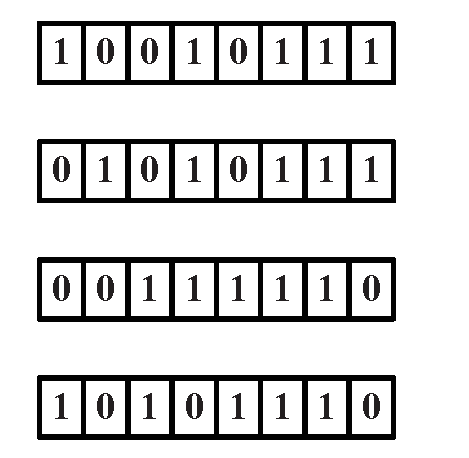
\includegraphics[width=1.3 in]{fig/spanding1}\label{fig:spanding1}}
%\subfigure[Expanding speed $\Im=2$]{\includegraphics[width=3.5 in]{fig/spanding2}\label{fig:spanding2}}
%\caption{SFBF with constant expanding speed.}
%\label{fig:SFBF with different expanding speed.}
%\end{figure}



\section{Performance evaluation}
\label{sec:simulation}
We first describe the experiment setup, then present the experiment results.
\subsection{Experiment setup}
We apply both real-world and synthetic data traces to comprehensively evaluate our proposed SFBF structure. Four data traces are used in the experiments:

\begin{itemize}
  \item MAWI \cite{MAWI}: This traffic data repository is maintained by the MAWI Working Group of the WIDE Project. The MAWI trace  contains 15 minutes of daily traffic captured from a trans-Pacific link between Japan and the United States. %The data are publicly available, and have the packet payloads omitted and IP addresses anonymous. Originated from January 2001, MAWI project currently maintains more than 14 years of traffic.
  \item Synthetic trace: All the data items in this trace are randomly generated within the range from 0 to $2^{32}-1$.
  \item Calgary-HTTP \cite{Calgary}: This trace contains the HTTP requests to the University of Calgary's Department of Computer Science WWW server located at Calgary, Alberta, Canada.
  \item NASA-HTTP \cite{NASA}: This trace contains two month's  HTTP requests to the NASA Kennedy Space Center WWW server in Florida.
\end{itemize}


For the first trace MAWI, we extract the Source IP address (32bit) from the MAWI trace  as the key  to insert into and query against the SFBF. For the Synthetic trace, the generated data item is directly used as the key to operate against the SFBF.
For the last two  traces, we apply MurMurhash's hash to the URL string to generate the 32 bit URL fingerprint,  which is used as the key to operate against the SFBF. %\note{Does MurMurhash's hash the shifting feature you introduced? }
The detailed information of traces used in this paper are shown in Table \ref{table:trace} .

\begin{table} [!htb]
\small
\newcommand{\tabincell}[2]{\begin{tabular}{@{}#1@{}}#2\end{tabular}}
    \newcommand{\specialcell}[2][c]{%
      \begin{tabular}[#1]{@{}c@{}}#2\end{tabular}}
    \centering
    \caption{Real Traffic Traces}
    \label{table:data_trace_table}
    \small
    \begin{tabular}{|c|c|c|}
        \hline
        data set &  data time &  No. Items  \\\hline
        \specialcell[c]{MAWI} & \specialcell[c]{2015-01-01\\ {[}14:00:01-14:00:15{]}} & 58066726  \\\hline
        %\specialcell[c]{MAWI 2} & \specialcell[c]{2015-2-21\\ {[}13:59:59-14:14:59{]}} & 58523738   \\\hline
        \specialcell[c]{Calgary-HTTP} & \specialcell[c]{{[}1995-08-28-00:00:00{]}\\ {[}1995-09-10-23:59:59{]}} & 3328587   \\\hline
        \specialcell[c]{NASA-HTTP} & \specialcell[c]{{[}1995-07-01-00:00:00{]}\\ {[}1995-08-31-23:59:59{]}} & 3461612   \\\hline
    \end{tabular}
    \label{table:trace}
\end{table}

Utilizing above traces, we perform a set of experiments to evaluate the performance of SFBF on a LENOVO workstation  equipped with Intel\textregistered {} Core\textsuperscript{TM} i5-5200U CPU (2.20GHz) and 8.00GB RAM. Each experiment dedicates to a specific SFBF, which is associated with randomly selected $k$ base hash generation matrices of dimension $32 \times 32$, i.e., the number of columns is $w=32$ and the number of rows is $R=32$. We set the number of columns in the base hash generation matrices to be 32, as the keys we use for all the trace cases are all 32 bits. That is, the IP address in MAWI trace is 32 bits, the URL fingerprint in traces Calgary-HTTP and NASA-HTTP is 32 bits, and the data in the Synthetic trace are generated within the range from 0 to $2^{32}-1$. The length and the capacity of the  baseline BF vector in SFBF are
set to $m_0 = 1024$ and $n_0 = 64$, respectively. The number of hash functions is set to $k = 6$.


Each experiment includes two steps:
\begin{enumerate}

\item Following the insertion operation in Algorithm \ref{alg:Insertion Operations}, we use an SFBF consisting of multiple BF vectors to represent the first $3 \times 10^4$ data items in the data trace, with data items  arriving sequentially.  $k$ hash functions are applied to each data item to set $k$ locations of the active BF vector to 1. Starting with the smallest baseline BF vector, when the data expands, SFBF expands and a new BF vector is created and added into SFBF if necessary with the filter length determined by the expanding speed $\lambda$. %\note{The trace data are static. You just simulated using some selected lambda variation patterns, rather letting the lambda changes according to the arrival speed as you claim. Isn't your design goal to change lambda according to the data arrival speed?}
    After all data items are represented by SFBF, the space usage of SFBF is known.

\item In order to evaluate the performance, after all data items in a data set have been represented by SFBF, we use another 150,000 data items in the traces to determine the false positive rates of SFBFs.  We run the querying Algorithm \ref{alg:Low cost query algorithm} using the same $k$ hash generation matrices in the insertion step. If the querying process returns true for a data item not in the set, it is counted as a filter false positive. The false positive rate for SFBF is the faction of $1.5 \times 10^5$ total queries that are false positive. We also insert a timer to measure the querying time.
\end{enumerate}



Besides SFBF, for performance comparison, we implement DBF proposed in~\cite{guo2006theory} which expands
the Bloom filter by adding a fixed-size BF vector each time as the data set becomes larger.  For each parameter combination, we repeat our experiments 100 times and take their average.

Moreover, as SFBF is designed to represent a dynamic data set, to evaluate the performance of SFBF under different expanding speeds, different $\lambda $ values are simulated to control the SFBF's expanding process.

\begin{itemize}
  \item $\lambda_1$: following the sequence: 1, 2, 3, 4, 5, 7, 9, ...
  \item $\lambda_2$: following the sequence: 1, 3, 5, 7, 9, 11, 13, ...
  \item $\lambda_3$: following the sequence: 1, 1, 2, 2, 3, 3, 4, 4,...
  \item $\lambda_4$: randomly  within $[1,3]$
  \item $\lambda_5$: randomly  within $[1,5]$
\end{itemize}

Under  $\lambda_1$, when the data set expands, the lengths of each vector added are  ${n_0},2{n_0},{2^2}{n_0},{2^3}{n_0}, \cdots$, so the vector length follows the exponential growth. Under  $\lambda_2$, the lengths of each vector added are  ${n_0},{2^2}{n_0},{2^4}{n_0}, {2^6}{n_0},\cdots$, where the vector length also follows the exponential growth but at a speed faster than that under $\lambda_1$. Under  $\lambda_3$, the lengths of each vector added are  ${n_0},{n_0}, 2{n_0},2{n_0},{2^2}{n_0},{2^2}{n_0},{2^3}{n_0}, {2^3}{n_0},\cdots$, which expands slower than that under  $\lambda_1$.  Under $\lambda_4$, the expanding speed is randomly generated within $[1,3]$. As a result, there are three different length vectors with  ${n_0},2{n_0},{2^2}{n_0}$. Similarly, under $\lambda_5$, there are five different length vectors with  ${n_0},2{n_0},{2^2}{n_0},{2^3}{n_0},{2^4}{n_0}$.
\subsection{Evaluation results}

To evaluate the performance of SFBF, four performance metrics are applied to evaluate the proposed SFBF:
\begin{itemize}
  \item  Extension round: the total number of extension rounds needed to represent the dynamic increasing data set.
  \item  False positive rate: defined as the ratio between the number
of data items indicated by a SFBF that they are inserted into the SFBF
even though they are not and the total number of the queried items.
  \item  Querying CPU time: the total CPU time consumed to query an item against an SFBF.
  \item Size of filter: the space usage to represent the dynamic increasing data set.
\end{itemize}

\subsubsection{Extension round}

\begin{figure}[!h]
\center
\subfigure[Synthetic]{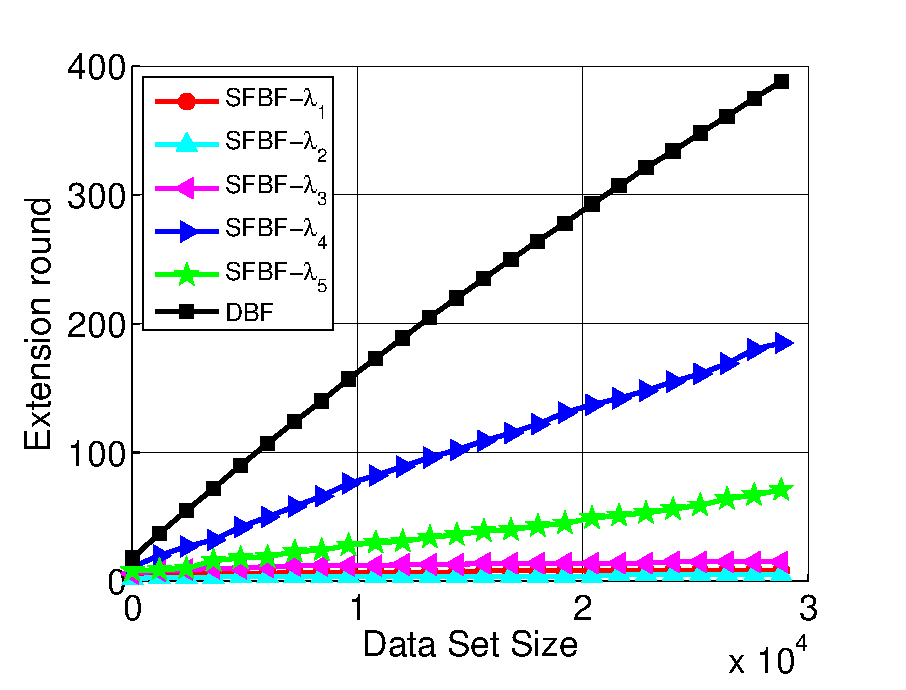
\includegraphics[width=1.45in]{franztao20160111/test1/Extensionround/test1_virtualdata}
\label{fig:Extension round test1 virtualdata.}}
\subfigure[MAWI]{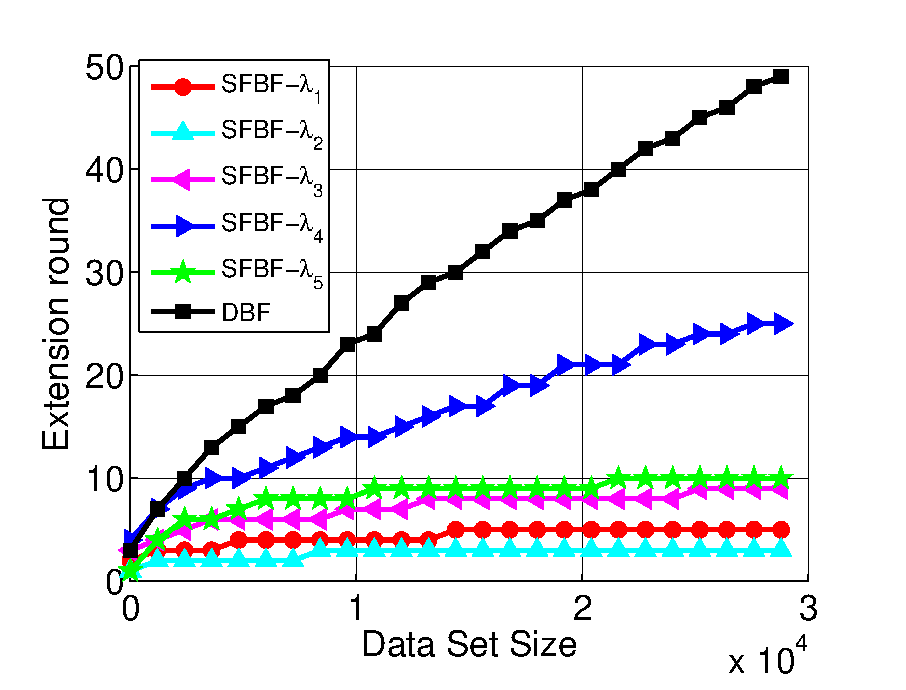
\includegraphics[width=1.45in]{franztao20160111/test1/Extensionround/test1_actualdata_IP_1}
\label{fig:Extension round test1_actualdataIP_1.}}
%\subfigure[MAWI 2]{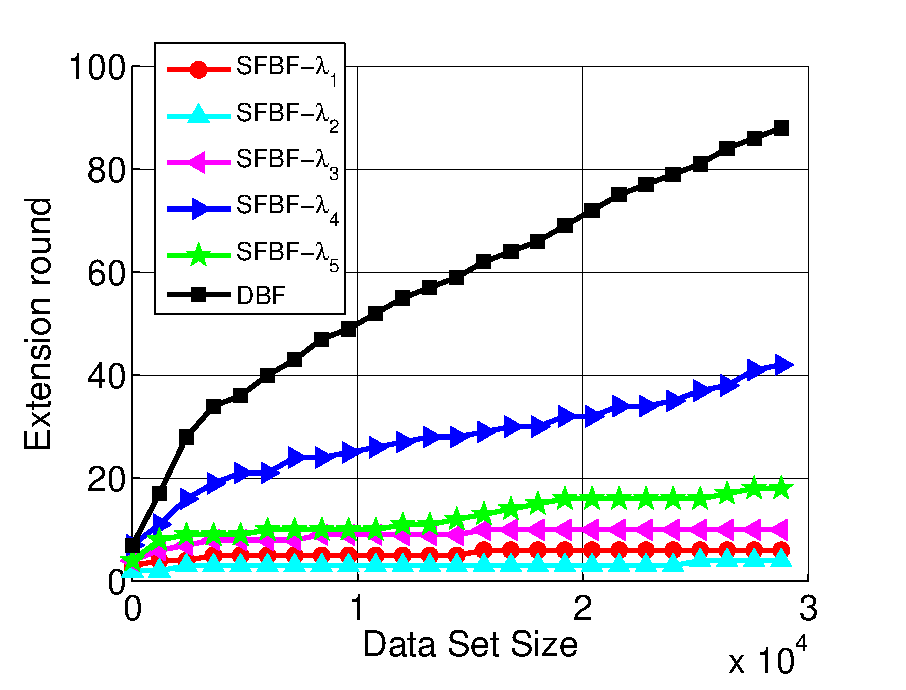
\includegraphics[width=1.4in]{franztao20160111/test1/Extensionround/test1_actualdata_IP_2}
%\label{fig:Extension round test1_actualdataIP_2.}}\\
\subfigure[Calgary-HTTP]{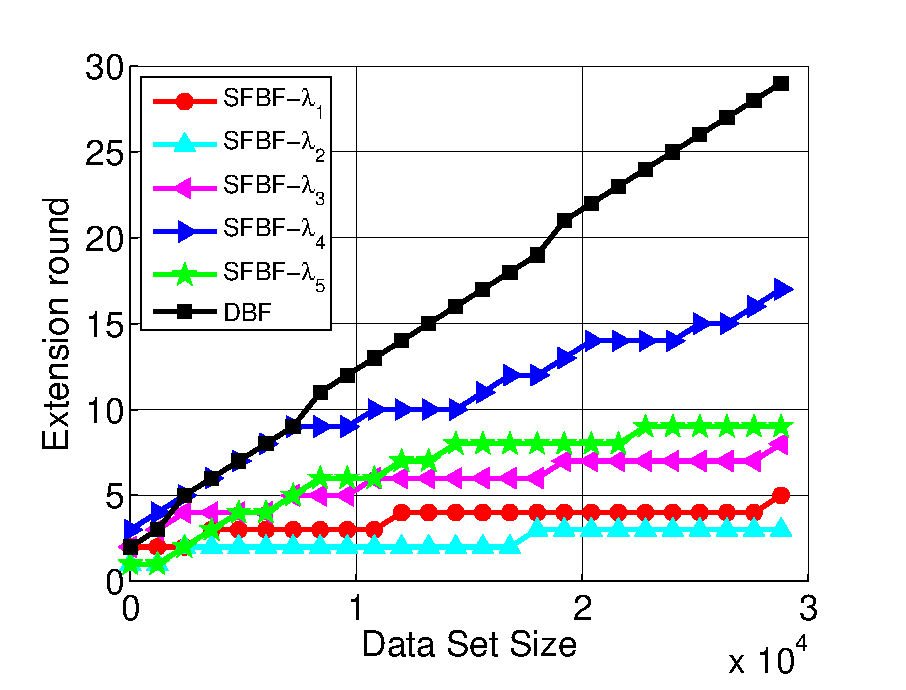
\includegraphics[width=1.45in]{franztao20160111/test1/Extensionround/test1_actualdata_webcache_1}
\label{fig:Extension round test1 actualdata webcache 1.}}
\subfigure[NASA-HTTP]{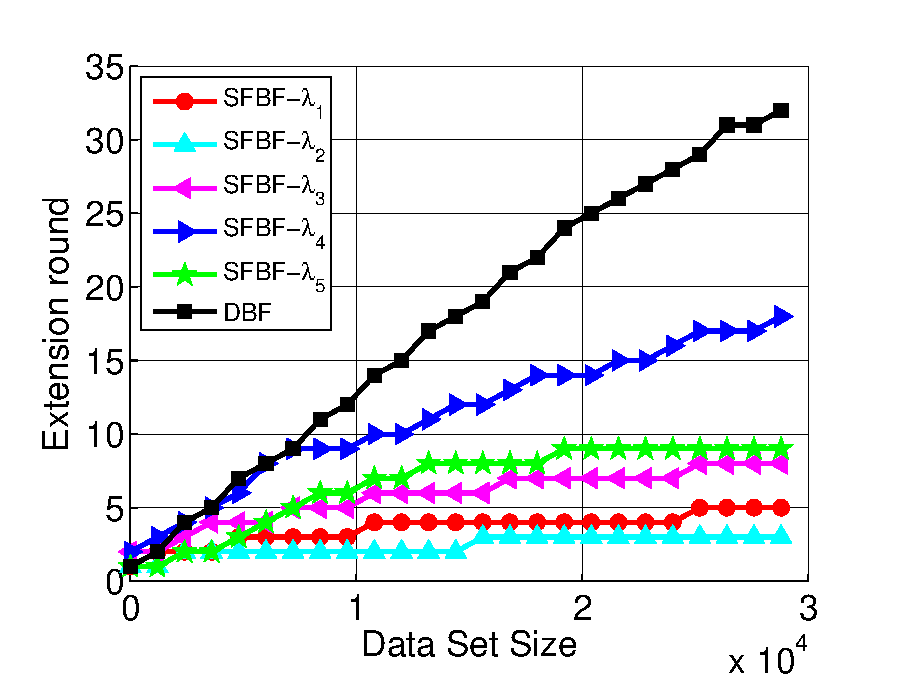
\includegraphics[width=1.45in]{franztao20160111/test1/Extensionround/test1_actualdata_webcache_2}
\label{fig:Extension round test1 actualdata webcache 2.}}
\caption{Extension round}
\label{fig:Extension round.}
\end{figure}

As discussed in the theoretical analysis, the expanding speed has an impact on the performance of an SFBF. The larger the expanding speed $\lambda$, the fewer the number of extension rounds needed for SFBF to represent a dynamic data set, as shown in Fig.\ref{fig:Extension round.}. This also indicates that the number of BF vectors in SFBF is also smaller, which allows for better performance with lower false positive rate and query CPU time, as shown in the next a few sections.

For the five implemented traces, at the same BF's parameter setting, the extension round under Synthetic trace is the largest among all other traces. All data items in the Synthetic trace are randomly generated which have a high probability to be unique, but many data items in other traces are duplicated (duplicated source IP address in  MAWI trace, and duplicated URL in Calgary-HTTP and NASA-HTTP traces). Therefore, even though the total number of data items to represent are the same, the total unique data items in the Synthetic trace are larger than those in other traces, which results in a larger extension round and higher false positive rate (in Fig.\ref{fig:False positive rate.}).

As shown in Fig.\ref{fig:Extension round.}, different from our SFBF, the extension procedures under DBF depends on the size of the data set, and the number of extension rounds increases about linearly with the size of data set.


%\note{Extension round is a metric, not an impact factor. So you should not put a separate section here. Your analysis is very messy. Metrics are what you should put on the Y axis, while impacts are what you should put on the X axis. I really don't know how you are analyzing data. For each impact, you are supposed to have one subsection, with multiple metrics shown associated with each impact.}



\subsubsection{False positive rate}

\begin{figure}[!h]
\center
\subfigure[Synthetic]{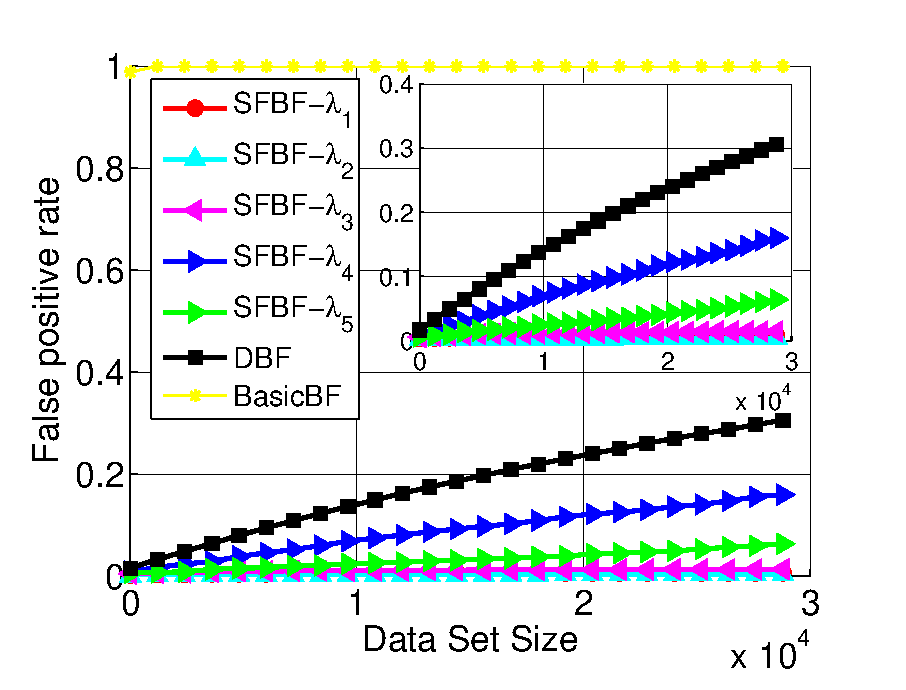
\includegraphics[width=1.45in]{franztao20160111/test1/Falsepositiverate/test1_virtualdata}
\label{fig:Falsepositiverate test1 virtualdata.}}
\subfigure[MAWI]{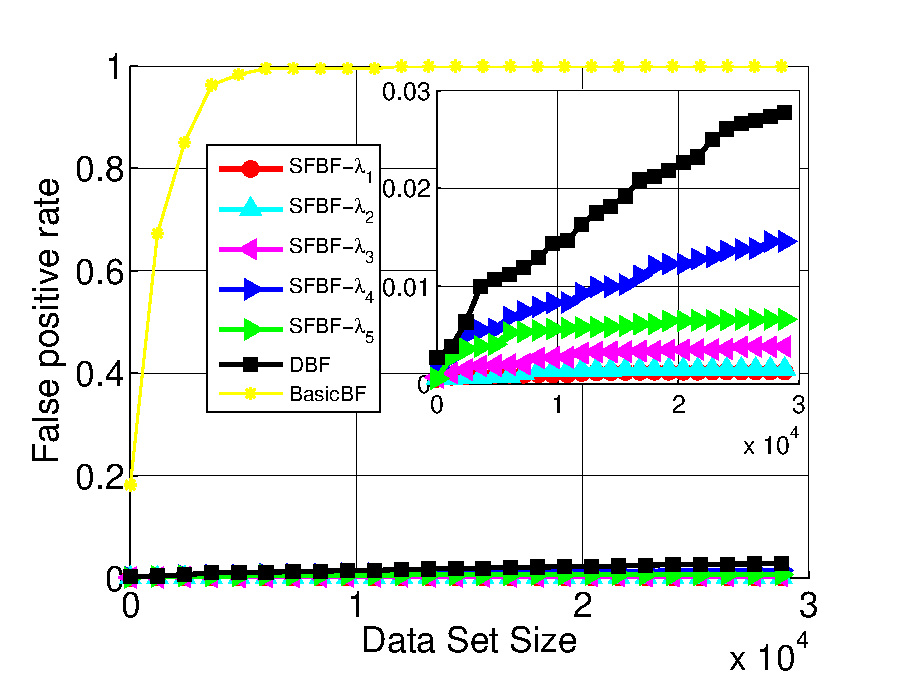
\includegraphics[width=1.45in]{franztao20160111/test1/Falsepositiverate/test1_actualdata_IP_1}
\label{fig:Falsepositiverate test1_actualdataIP_1.}}
%\subfigure[MAWI 2]{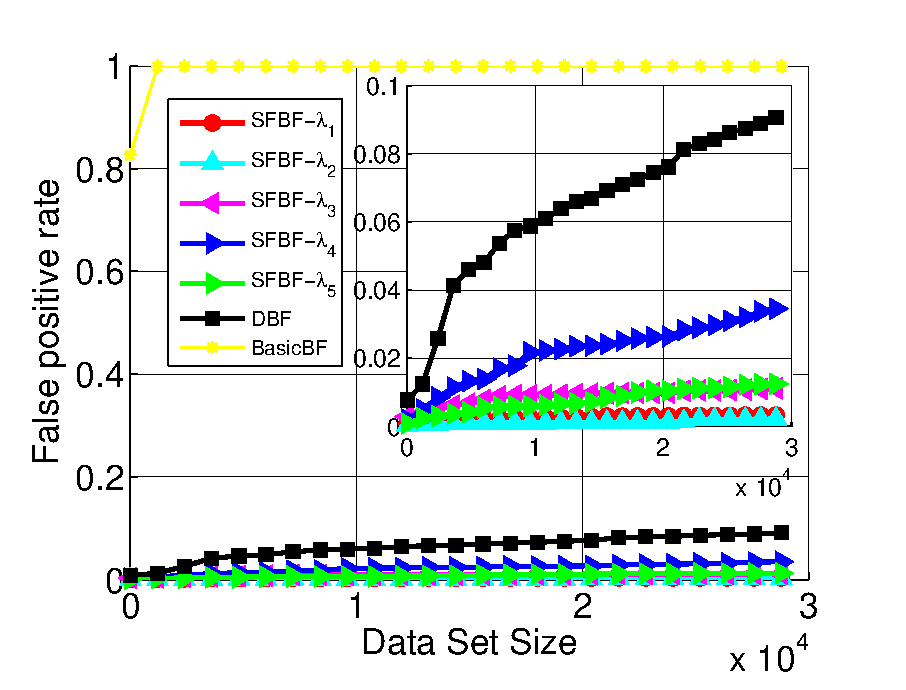
\includegraphics[width=1.4in]{franztao20160111/test1/Falsepositiverate/test1_actualdata_IP_2}
%\label{fig:Falsepositiverate test1_actualdataIP_2.}}\\
\subfigure[Calgary-HTTP]{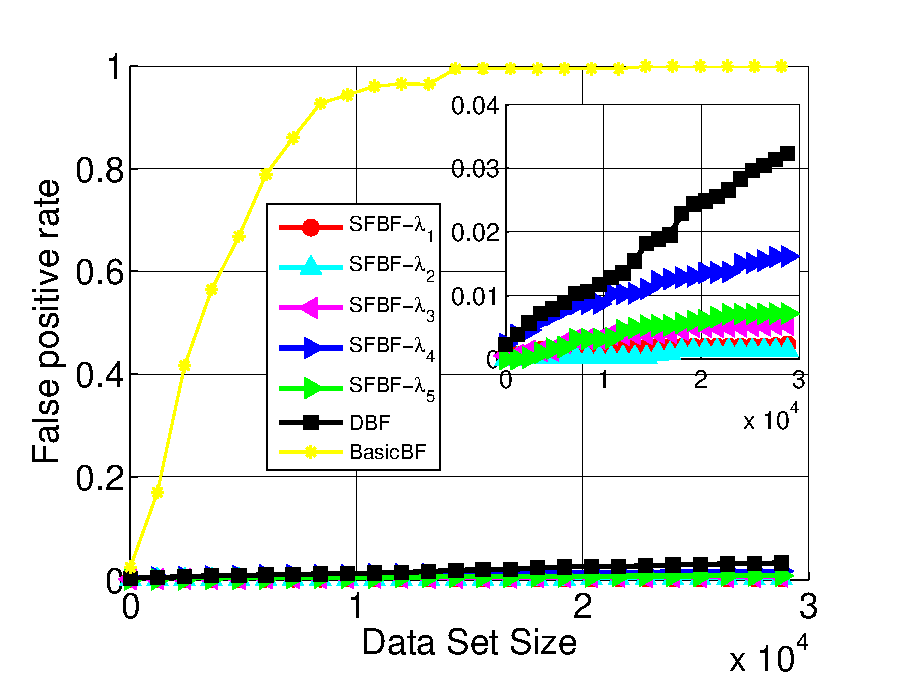
\includegraphics[width=1.45in]{franztao20160111/test1/Falsepositiverate/test1_actualdata_webcache_1}
\label{fig:Falsepositiverate test1 actualdata webcache 1.}}
\subfigure[NASA-HTTP]{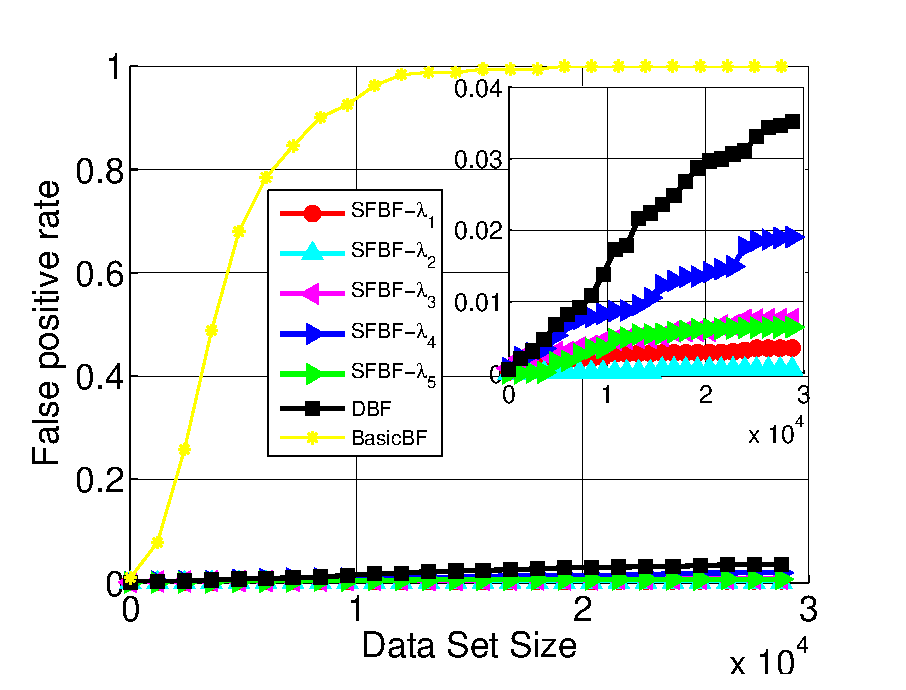
\includegraphics[width=1.45in]{franztao20160111/test1/Falsepositiverate/test1_actualdata_webcache_2}
\label{fig:Falsepositiverate test1 actualdata webcache 2.}}
\caption{False positive rate}
\label{fig:False positive rate.}
\end{figure}


%\begin{table*}[t]
%\footnotesize
%  \centering
%  \caption{False positive rate under SFBF}
%    \begin{tabular}{rrrr}
%        \toprule
%    \multirow{2}[4]{*}{Data Size(n)} & \multirow{2}[4]{*}{Hash function k} & \multicolumn{2}{r}{SFBF false positive rate}  \\
%          &       & Experiment  & Calculated  \\
%    %\toprule
%%    $Data Size(n)$ & $Hash function k$ & $Experiment result$ & $Calculated result$  \\
%          \midrule
%     \multirow{3}[4]{*}{2,000} & 6     & 0.00285 & 0.0024655  \\
%          & 8     & 0.00143 & 0.00147624  \\
%          & 11    & 0.0011 & 0.00114505  \\
%    \multirow{3}[4]{*}{4,000} & 6     & 0.00686 & 0.00652735  \\
%          & 8     & 0.00385 & 0.00401455  \\
%          & 11    & 0.00318 & 0.00320656  \\
%    \multirow{3}[4]{*}{6,000} & 6     & 0.01634 & 0.0155252  \\
%          & 8     & 0.00932 & 0.00953349  \\
%          & 11    & 0.00729 & 0.00759046  \\
%    \multirow{3}[4]{*}{8,000} & 6     & 0.02544 & 0.0249436  \\
%          & 8     & 0.01499 & 0.0153961  \\
%          & 11    & 0.01239 & 0.0123116  \\
%    \multirow{3}[4]{*}{10,000} & 6     & 0.02893 & 0.0285906  \\
%          & 8     & 0.01738 & 0.0176576  \\
%          & 11    & 0.01408 & 0.0141227  \\
%    \multirow{3}[4]{*}{12,000} & 6     & 0.0728476 & 0.0294973  \\
%          & 8     & 0.01804 & 0.0182216  \\
%          & 11    & 0.01461 & 0.0145749  \\
%    \multirow{3}[4]{*}{14,000} & 6     & 0.03156 & 0.0313076  \\
%          & 8     & 0.01915 & 0.0193488  \\
%          & 11    & 0.01542 & 0.0154787  \\
%    \multirow{3}[4]{*}{16,000} & 6     & 0.03242 & 0.0322134  \\
%          & 8     & 0.01978 & 0.0199122  \\
%          & 11    & 0.01588 & 0.0159303  \\
%    \bottomrule
%    \end{tabular}%
%  \label{tab:3}%
%\end{table*}
To illustrate the false positive rates under different Bloom Filter schemes, besides DBF and SFBF, Fig.\ref{fig:False positive rate.} also shows the curve of basic Bloom filter (denoted as BasicBF). As the data set expands to \DataSetSize, the false positive rate increases under all BF schemes. With the continuous increase of the set size $n$, the false positive rate of BasicBF approaches 1 rapidly, while our SFBF with all various expanding speed $\lambda$ can well control the false positive rate to remain at very low level.

In the small figure of Fig.\ref{fig:False positive rate.}, the curve of BasicBF is removed so DBF and SFBF can be more clearly represented. According to Eq.(\ref{eq:SFBFfalse positive}), the false positive ratio increases monotonically with the number of extension rounds. Thus, it will be smaller when the expanding speed $\lambda$ is raised to reduce the extension rounds.




When the data set expands to $n = $\DataSetSize, which is 388 times that of $n_0= 64$, the false positive rate of DBF reaches 30.59\% (for the Synthetic trace in Fig.\ref{fig:Falsepositiverate test1 virtualdata.}),
% the false positive rates of SFBF-$\lambda_1$ reach 0.69\% (in Synthetic trace in Fig.\ref{fig:Falsepositiverate test1 virtualdata.}),the false positive rates of SFBF-$\lambda_2$ reach 0.35\% (in Synthetic trace in Fig.\ref{fig:Falsepositiverate test1 virtualdata.}),the false positive rates of SFBF-$\lambda_3$ reach 1.3\% (in Synthetic trace in Fig.\ref{fig:Falsepositiverate test1 virtualdata.}),the false positive rates of SFBF-$\lambda_4$ reach 16.0\% (in Synthetic trace in Fig.\ref{fig:Falsepositiverate test1 virtualdata.}),the false positive rates of SFBF-$\lambda_5$ reach 6.38\% (in Synthetic trace in Fig.\ref{fig:Falsepositiverate test1 virtualdata.})
   which makes it not usable. The results indicate that DBF is not really scalable.






\subsubsection{Querying CPU time}
\begin{figure}[!h]
\center
\subfigure[Synthetic]{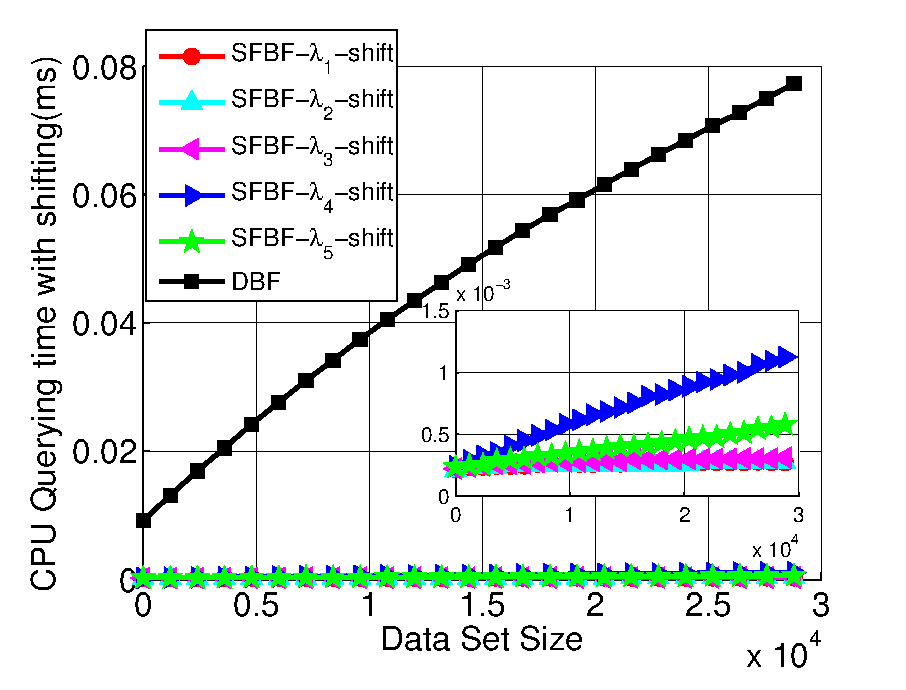
\includegraphics[width=1.45in]{franztao20160111/test1/QueryingCPUtimewithshifting/test1_virtualdata}
\label{fig:QueryingCPUtimewithshifting test1 virtualdata.}}
\subfigure[MAWI]{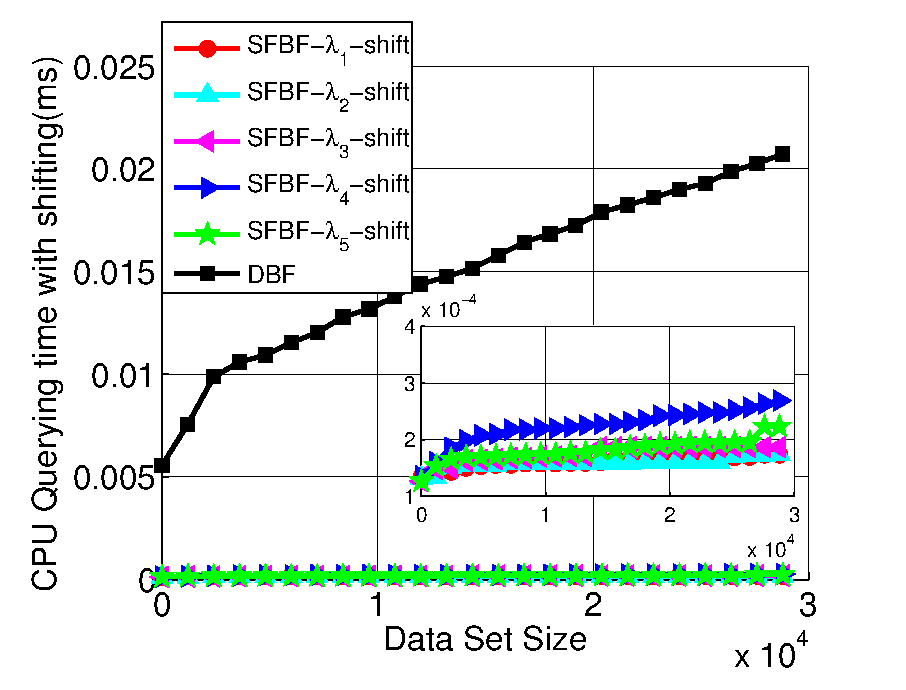
\includegraphics[width=1.45in]{franztao20160111/test1/QueryingCPUtimewithshifting/test1_actualdata_IP_1}
\label{fig:QueryingCPUtimewithshifting test1_actualdataIP_1.}}
%\subfigure[MAWI 2]{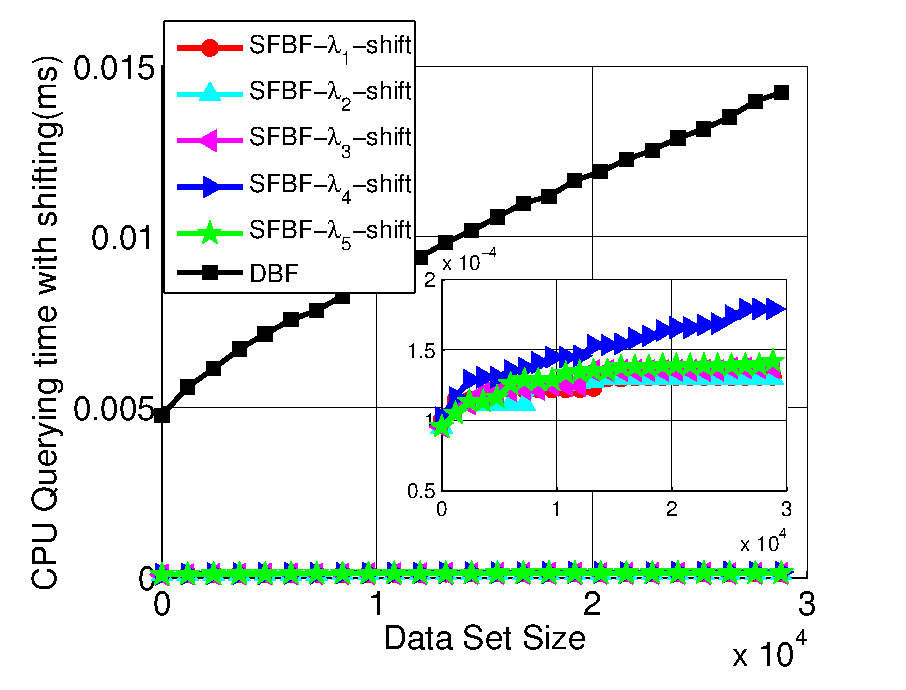
\includegraphics[width=1.4in]{franztao20160111/test1/QueryingCPUtimewithshifting/test1_actualdata_IP_2}
%\label{fig:QueryingCPUtimewithshifting test1_actualdataIP_2.}}\\
\subfigure[Calgary-HTTP]{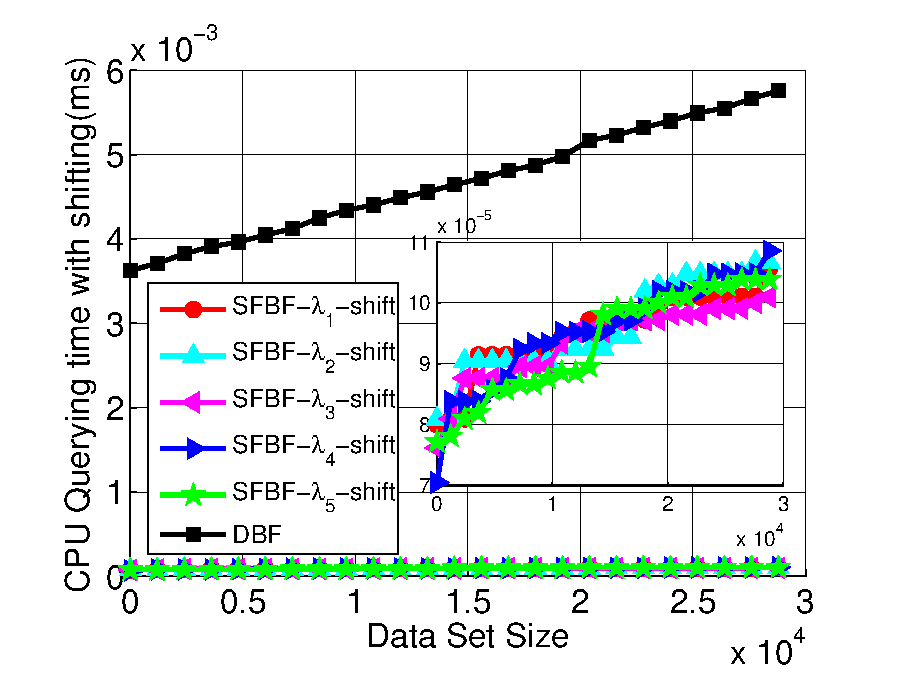
\includegraphics[width=1.45in]{franztao20160111/test1/QueryingCPUtimewithshifting/test1_actualdata_webcache_1}
\label{fig:QueryingCPUtimewithshifting test1 actualdata webcache 1.}}
\subfigure[NASA-HTTP]{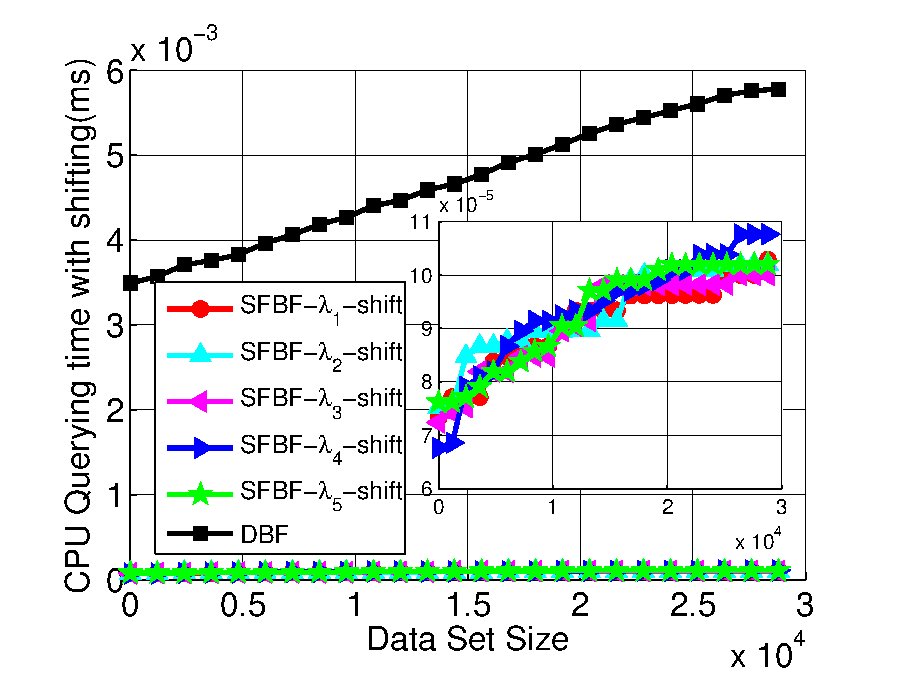
\includegraphics[width=1.45in]{franztao20160111/test1/QueryingCPUtimewithshifting/test1_actualdata_webcache_2}
\label{fig:QueryingCPUtimewithshifting test1 actualdata webcache 2.}}
\caption{Querying CPU time with shifting}
\label{fig:Querying CPU time with shifting.}
\end{figure}



\begin{figure}[!h]
\center
\subfigure[Synthetic]{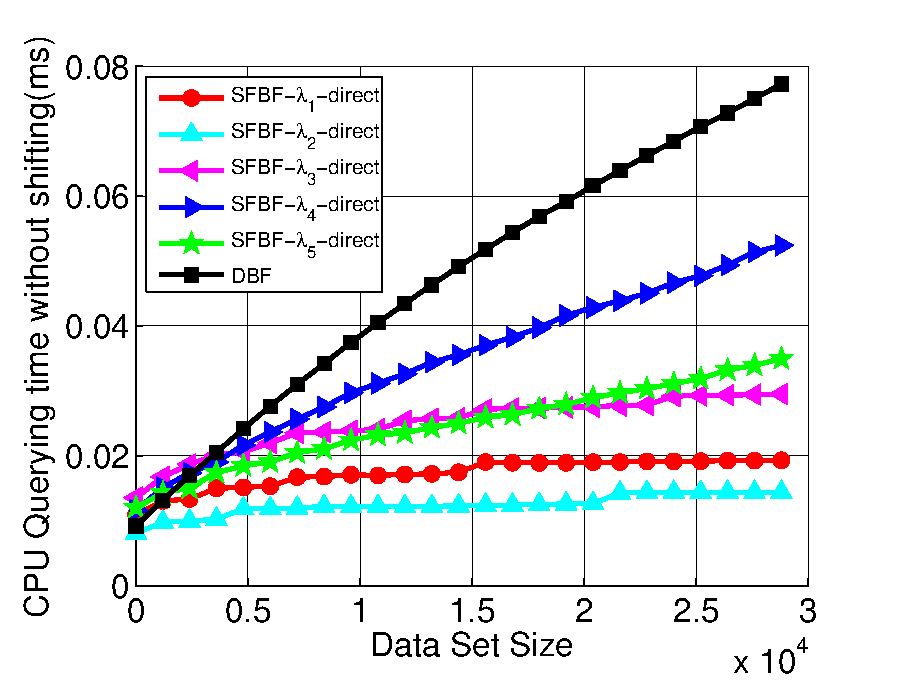
\includegraphics[width=1.45in]{franztao20160111/test1/QueryingCPUtimewithoutshifting/test1_virtualdata}
\label{fig:QueryingCPUtimewithoutshifting test1 virtualdata.}}
\subfigure[MAWI]{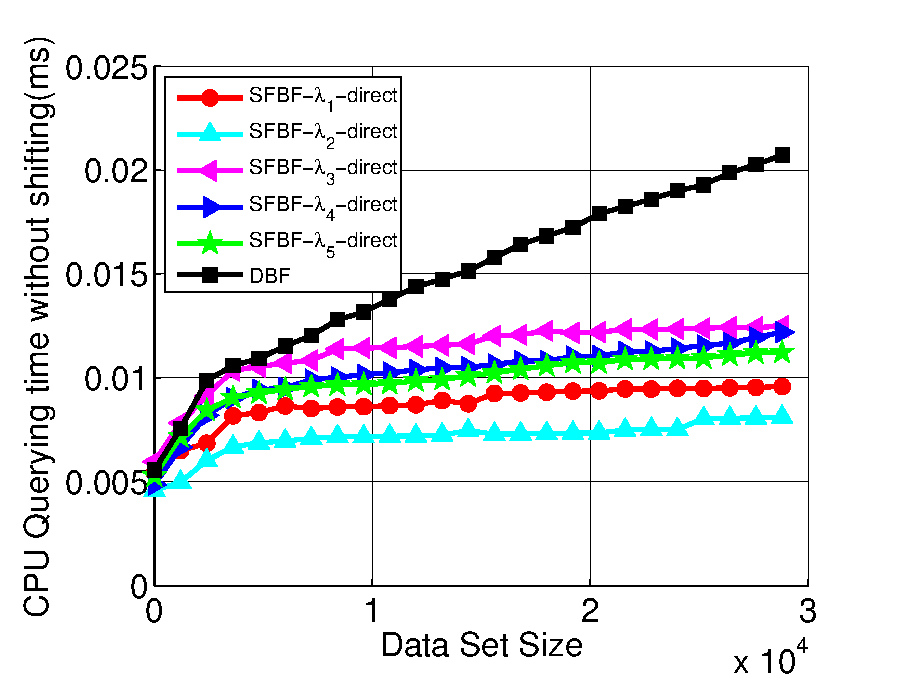
\includegraphics[width=1.45in]{franztao20160111/test1/QueryingCPUtimewithoutshifting/test1_actualdata_IP_1}
\label{fig:QueryingCPUtimewithoutshifting test1_actualdataIP_1.}}
%\subfigure[MAWI 2]{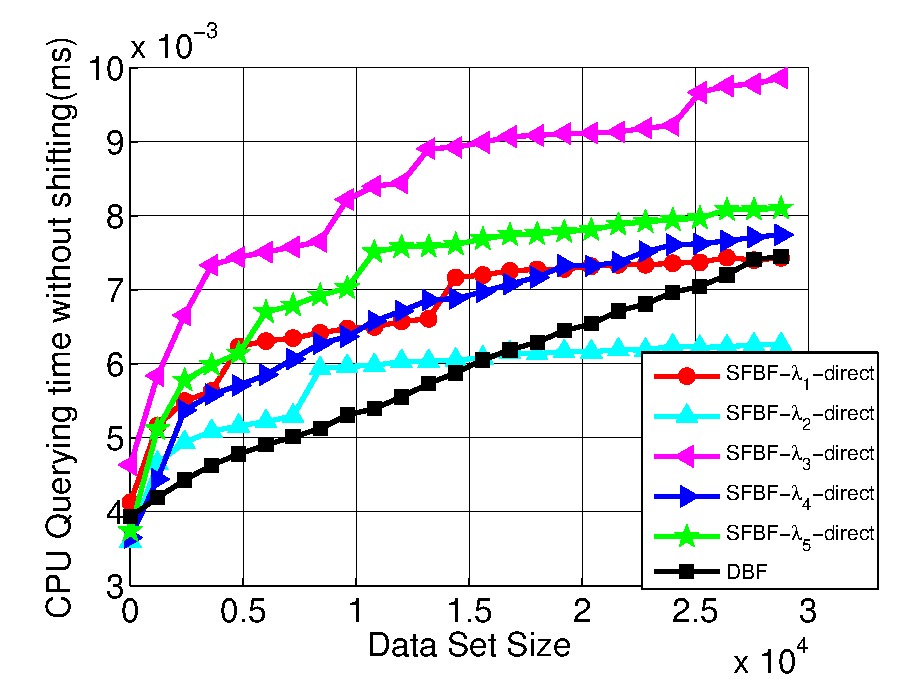
\includegraphics[width=1.4in]{franztao20160111/test1/QueryingCPUtimewithoutshifting/test1_actualdata_IP_2}
%\label{fig:QueryingCPUtimewithoutshifting test1_actualdataIP_2.}}\\
\subfigure[Calgary-HTTP]{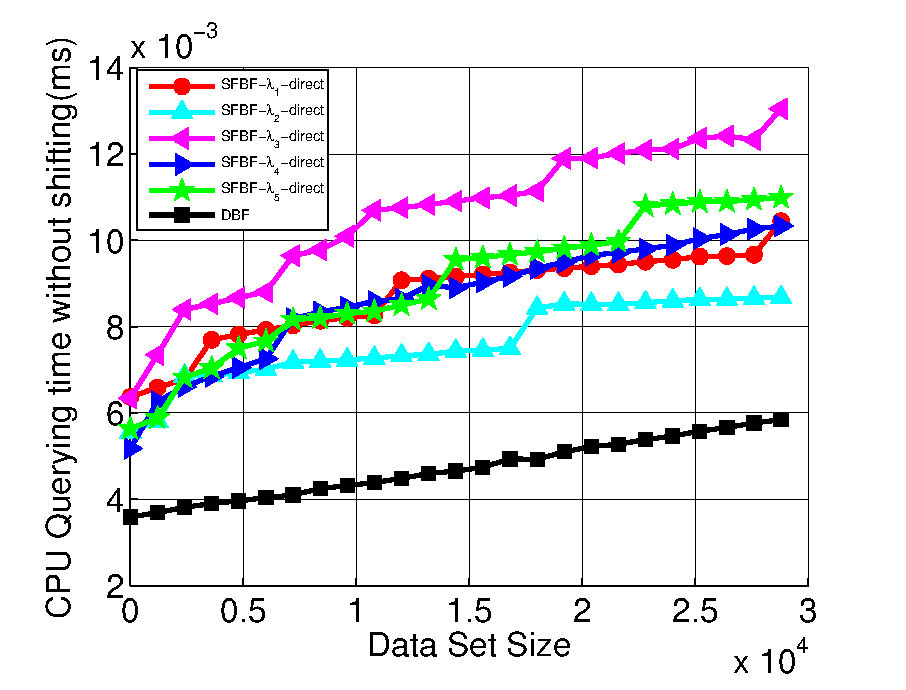
\includegraphics[width=1.45in]{franztao20160111/test1/QueryingCPUtimewithoutshifting/test1_actualdata_webcache_1}
\label{fig:QueryingCPUtimewithoutshifting test1 actualdata webcache 1.}}
\subfigure[NASA-HTTP]{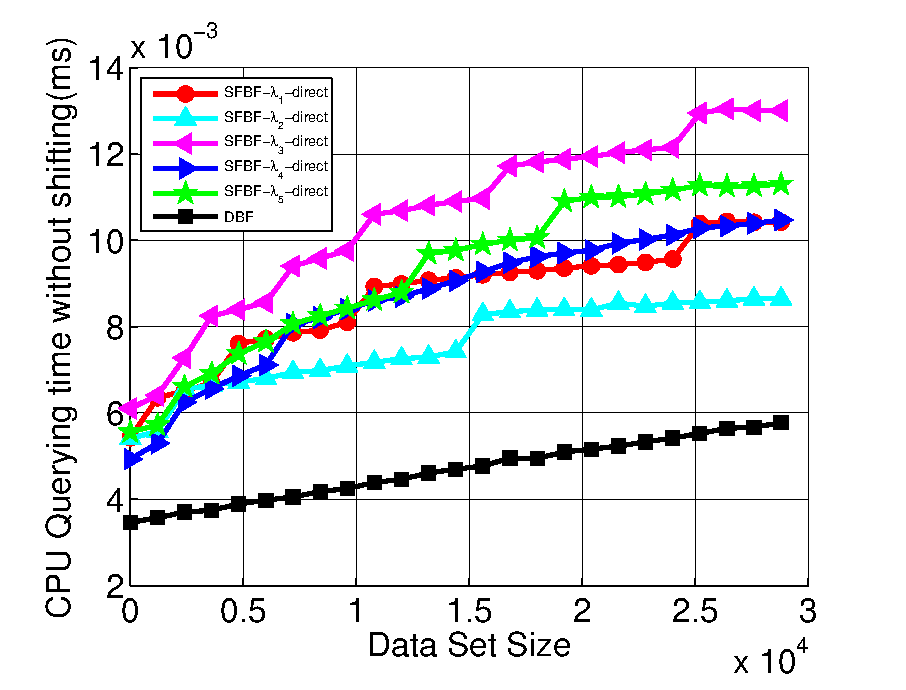
\includegraphics[width=1.45in]{franztao20160111/test1/QueryingCPUtimewithoutshifting/test1_actualdata_webcache_2}
\label{fig:QueryingCPUtimewithoutshifting test1 actualdata webcache 2.}}
\caption{Querying CPU time without shifting}
\label{fig:Querying CPU time without shifting.}
\end{figure}




Fig.\ref{fig:Querying CPU time with shifting.} and Fig.\ref{fig:Querying CPU time without shifting.} compare the query time among different BF designs. In order to find the longest query time, besides the first \DataSetSize data items, additional \SearchDataSize data items in the traces are used to query against the bloom filters. We run 100 times to get the average results. DBF consists of BF vectors with the same length, while our SFBF consists of BF vectors with varying filter length.

For SFBF, we implement two query schemes to handle the varying filter length, a query algorithm with the shifting operation (denoted as Shift) as shown in Fig.\ref{fig:Querying CPU time with shifting.}, and a query algorithm with the direct hash computation (denoted as Direct) as shown in Fig.\ref{fig:Querying CPU time without shifting.}. In the first scheme, when querying an element against a BF array with multiple BF vectors, we execute one set of hash computations for the $k$ hash functions over the largest BF vector, and then take the bit shifting operation to obtain the corresponding addresses of element to query in other BF vectors. In the second scheme, when querying a data item against a BF array, every same-length-BF-vector needs one set of hash computations for $k$ hash functions. Because DBF consists of multiple BF vectors with the same filter length, its  hash addresses for the element queried in all BF vectors are the same and only one set of hash computations with $k$ hash functions is needed. For performance comparison, we draw the curve of DBF in both Fig.\ref{fig:Querying CPU time with shifting.} and Fig.\ref{fig:Querying CPU time without shifting.}.


 Comparing the Shifting scheme in Fig.\ref{fig:Querying CPU time with shifting.}  with the Direct scheme in Fig.\ref{fig:Querying CPU time without shifting.}, obviously, our Shift scheme proposed is very efficient and effective in largely reducing the query CPU time. Taking the trace MAWI for example, when the data set expands to \DataSetSize, the average querying CPU time under SFBF-$\lambda_1$-Shift, SFBF-$\lambda_2$-Shift, SFBF-$\lambda_3$-Shift, SFBF-$\lambda_4$-Shift, SFBF-$\lambda_5$-Shift, and are only 1.8\%, 2.2\%, 1.5\%, 2.2\% and 2.0\% of those under SFBF-$\lambda_1$-Direct, SFBF-$\lambda_2$-Direct, SFBF-$\lambda_3$-Direct, SFBF-$\lambda_4$-Direct and SFBF-$\lambda_5$-Direct.

The query time of DBF consists of hash function computation time and comparison time while the later depends on the total number of extension rounds. The query CPU time of SFBF consists of the hash function computation time, comparison time, and shifting time, among which the later two depend on the total number of extension rounds.

 Compared to DBF, our SFBF can well control the extension round even when the data set is expanded to a very large size, as shown in Fig.\ref{fig:Extension round.}, therefore the increase of querying time in DBF is much faster than SFBF when the set expands, as shown in Fig.\ref{fig:Querying CPU time with shifting.}. When the data set expands to \DataSetSize, DBF needs much more CPU time than those of SFBF, as shown in Fig.\ref{fig:Querying CPU time with shifting.}. Take the trace MAWI as an example, the average query time of DBF is 0.021 ms, while the time of SFBF-$\lambda_1$-Shift, SFBF-$\lambda_2$-Shift, SFBF-$\lambda_3$-Shift, SFBF-$\lambda_4$-Shift, and SFBF-$\lambda_5$-Shift are $0.1733 \times 10^{-3}$ ms, $0.1744 \times 10^{-3}$ ms, $0.1869 \times 10^{-3}$ ms, $0.2689 \times 10^{-3}$ and $0.2233 \times 10^{-3}$ ms, respectively. This also   demonstrates that our shifting operation is  very
efficient and effective in largely reducing the query CPU time.

It is noted that querying a data item  only takes  less than $0.2 \times 10^{-3}$ ms for a query in a 2.20GHz computer, which is quite acceptable.
%\note{You need to explain why, not to simply how values. Is the extension number much smaller? Dear sister, the main resons that our SFBF is much lower than DBF is that the shifting is very efficient and effective. I have added the reasons. }

For the different traces, the query time under the Synthetic trace are much larger than other traces. To query a data item not presented by the SFBF, all the BF vectors should be checked unless a false positive happens.
Thus, a data set requiring a larger number of BF vectors would lead to a large query time. As data items in the Synthetic trace have a high probability of being  unique, it requires more BF vectors to represent the corresponding data set.  In addition,  data in other traces have more duplicated items, so their query hit ratios are larger than that in the Synthetic trace. When there is a query hit, it does not need to check all the BF vectors, which would also result in a smaller query time.



\subsubsection{Size of filter}

\begin{figure}[!h]
\center
\subfigure[Synthetic]{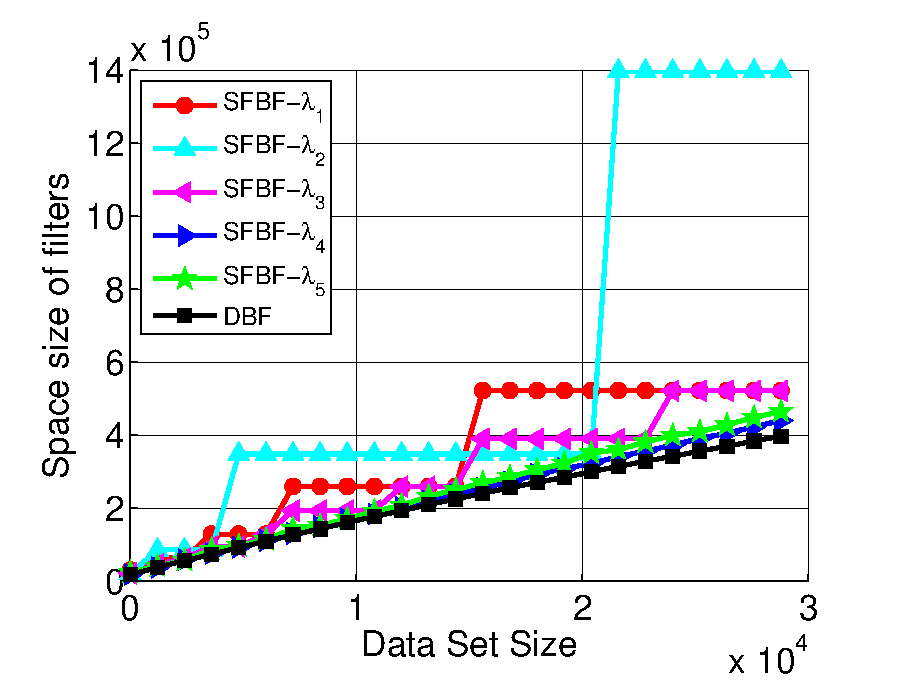
\includegraphics[width=1.45in]{franztao20160111/test1/Spacesizeoffilters/test1_virtualdata}
\label{fig:Spacesizeoffilters test1 virtualdata.}}
\subfigure[MAWI]{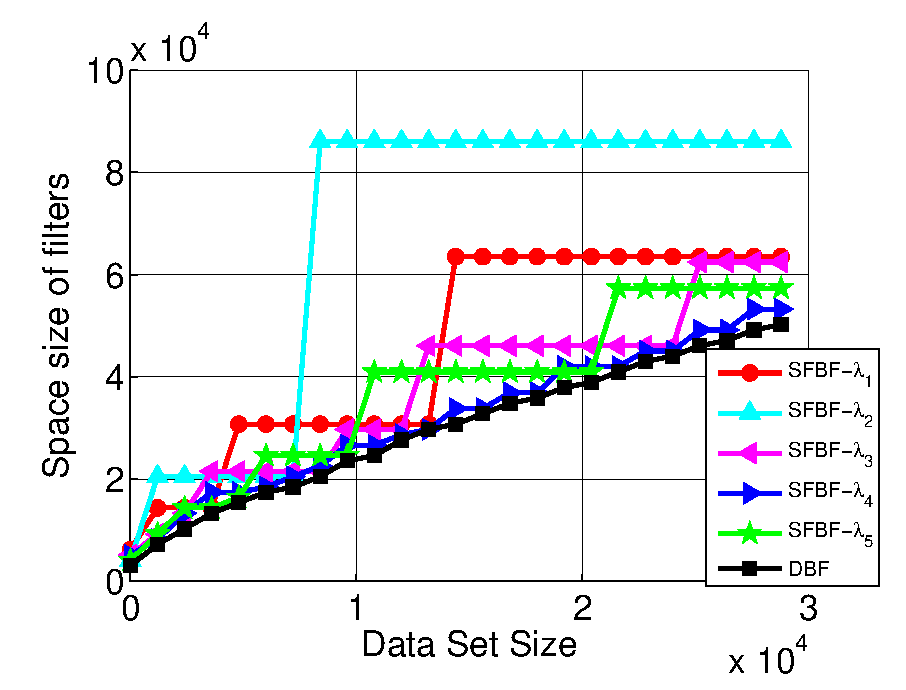
\includegraphics[width=1.45in]{franztao20160111/test1/Spacesizeoffilters/test1_actualdata_IP_1}
\label{fig:Spacesizeoffilters test1_actualdataIP_1.}}
%\subfigure[MAWI 2]{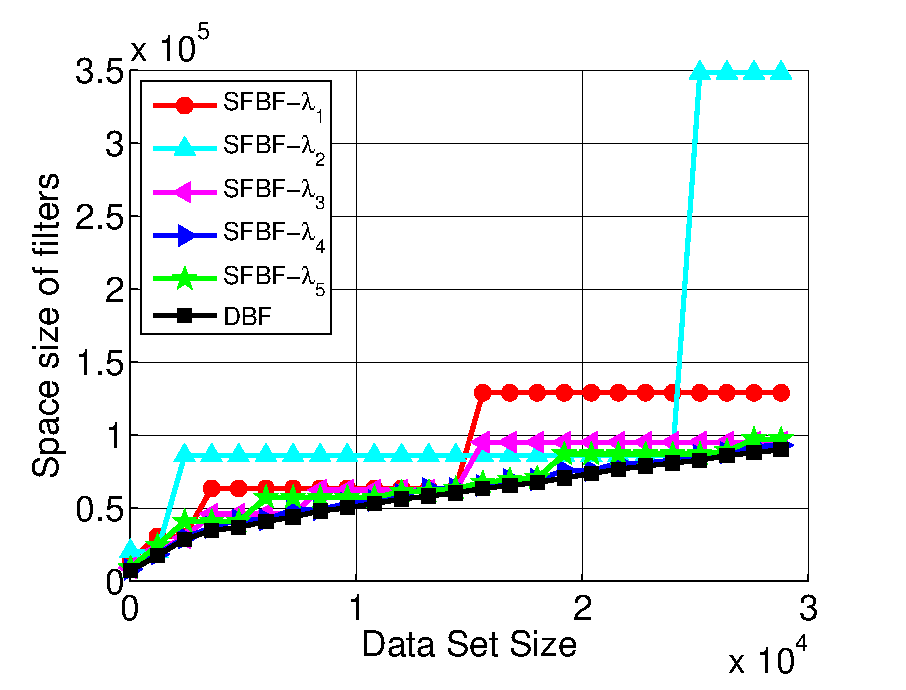
\includegraphics[width=1.4in]{franztao20160111/test1/Spacesizeoffilters/test1_actualdata_IP_2}
%\label{fig:Spacesizeoffilters test1_actualdataIP_2.}}\\
\subfigure[Calgary-HTTP]{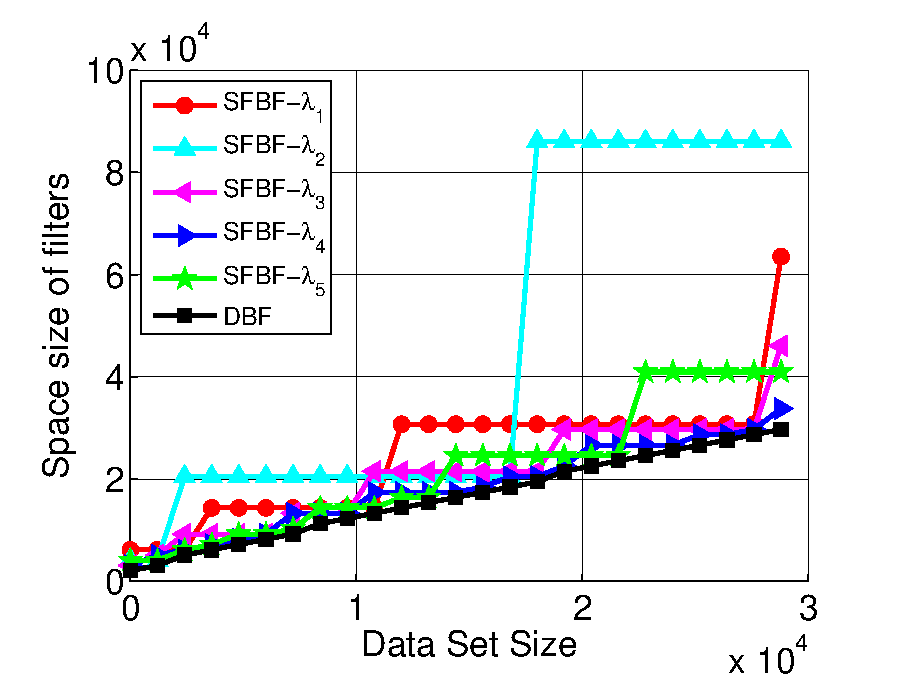
\includegraphics[width=1.45in]{franztao20160111/test1/Spacesizeoffilters/test1_actualdata_webcache_1}
\label{fig:Spacesizeoffilters test1 actualdata webcache 1.}}
\subfigure[NASA-HTTP]{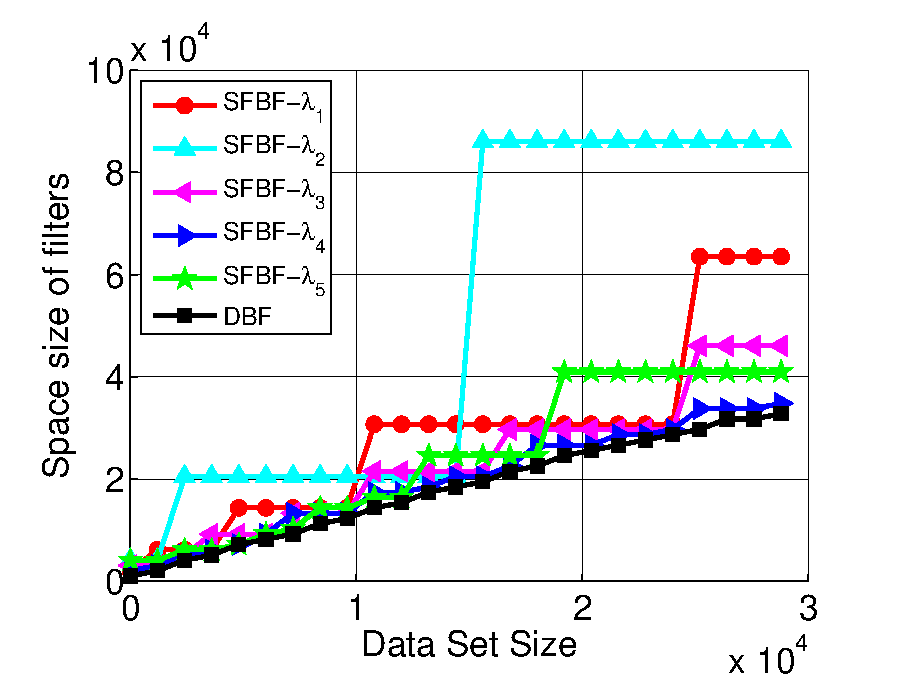
\includegraphics[width=1.45in]{franztao20160111/test1/Spacesizeoffilters/test1_actualdata_webcache_2}
\label{fig:Spacesizeoffilters test1 actualdata webcache 2.}}
\caption{Space size of filters}
\label{fig:Space size of filters.}
\end{figure}



Fig.\ref{fig:Space size of filters.} compares different Bloom filter designs in term of space usage.
Take the trace Synthetic as an example (in Fig.\ref{fig:Spacesizeoffilters test1 virtualdata.}) , as the data set expands, the curves of DBF, SFBF-$\lambda_1$, SFBF-$\lambda_2$, SFBF-$\lambda_3$, SFBF-$\lambda_4$, SFBF-$\lambda_5$ increase in the form of ladders with different width, while the DBF ladder has the same width for each level.
The width in a ladder level denotes the maximum number of data items that can be represented by the corresponding BF vector, which depends on the expanding speed in our SFBF design.

Take the trace MAWI as an example, when the data set expands to \DataSetSize, even though the space usage under DBF, SFBF-$\lambda_1$,  SFBF-$\lambda_3$, SFBF-$\lambda_4$ and SFBF-$\lambda_5$ is close, the false positive rates of SFBF-$\lambda_1$,  SFBF-$\lambda_3$, SFBF-$\lambda_4$ and SFBF-$\lambda_5$ are only 4.67\%,  13.82\%, 52.58\%, and 23.87\% of that of DBF, and the query time of SFBF-$\lambda_1$-Shift,  SFBF-$\lambda_3$-Shift, SFBF-$\lambda_4$-Shift, SFBF-$\lambda_5$-Shift are 0.83\%, 0.84\%, 0.90\%, and 1.30\% of that of DBF, as can be seen from Fig.\ref{fig:Falsepositiverate test1_actualdataIP_1.} and Fig.\ref{fig:QueryingCPUtimewithshifting test1_actualdataIP_1.}.
In summary, the performance results demonstrate that SFBF can well control the false positive rate to be at very low level and low query CPU time even when the data set expands to very large size.




\section{Conclusion}
\label{sec:CONCLUSION}
A Bloom Filter (BF) is a space-efficient probabilistic data structure allowing membership queries over
sets with certain allowable errors. It is widely used in many applications which take advantage of
its ability to compactly represent a set, and filter out effectively any element that does not belong
to the set. However, efficiency and scalability becomes big challenge in applying BF to a big data environment in which large scale and ever-increasing data arrive unpredictably. This paper proposes a  Scalable and Flexible Bloom
filter (SFBF) to address the scalability issue of Bloom filters. Specifically, we propose a novel algorithm to adaptively generate hash functions and a light-weight SFBF query algorithm that takes advantage of the features of our proposed hash functions to ensure light-weight member matching in a dynamic big data environment. Bloom filters and related variants have found many applications. It is expected that SFBF is applicable in many practical systems with constant changes of the number of members in a set.

\bibliographystyle{ieeetr}
\bibliography{LB_Offload_in_MC}
%\bibliography{JointFlowRouting}
\begin{IEEEbiography}[{
\includegraphics[width=1in,height=1.25in,clip,keepaspectratio]{fig/kunxie}}]{Kun Xie}
received PhD degree in computer application from Hunan University, Changsha, China,
in 2007. She worked as a postdoctoral fellow
in the department of computing in Hong Kong Polytechnic University from
2007.12 to 2010.2. She worked as a visiting researcher in the department
of electrical and computer engineering in state university of New York at
Stony Brook from 2012.9 to 2013.9.
Her research interests include wireless network and mobile
computing, network management and control, cloud computing and mobile
cloud, and big data.
\end{IEEEbiography}
\begin{IEEEbiography}[{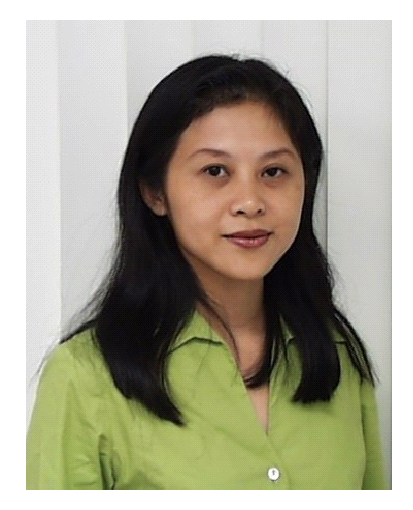
\includegraphics[width=1in,height=1.25in,clip,keepaspectratio]{fig/xinwang}}]{Xin Wang}
 received the Ph.D. degree in electrical and computer engineering from Columbia University, New York, NY.
She is currently an Associate Professor in the Department of Electrical and Computer Engineering of the State University of New York at Stony Brook, Stony Brook, NY. Before joining Stony Brook, she was a Member of Technical Staff in the area of mobile and wireless networking at Bell Labs Research, Lucent Technologies, New Jersey, and an Assistant Professor in the Department of Computer Science and Engineering of the State University of New York at Buffalo, Buffalo, NY. Her research interests include algorithm and protocol design in wireless networks and communications, mobile and distributed computing, as well as networked sensing and detection. She has served in executive committee and technical committee of numerous conferences and funding review panels, and served as the associate editor of IEEE Transactions on Mobile Computing. Dr. Wang achieved the NSF career award in 2005, and ONR challenge award in 2010.
\end{IEEEbiography}

\begin{IEEEbiography}[{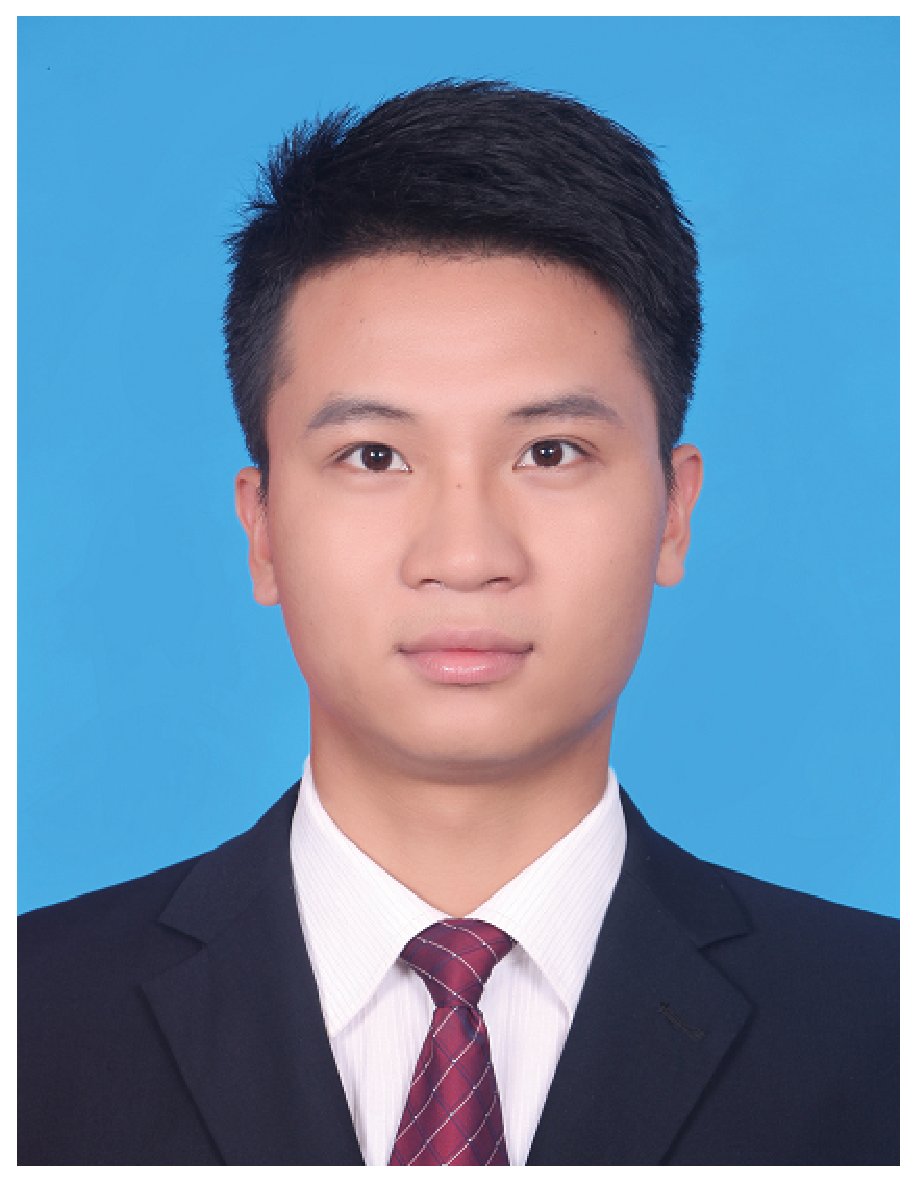
\includegraphics[width=1in,height=1.25in,clip,keepaspectratio]{fig/taoheng}}]{Heng Tao}
 is now a master student in the department of electrical and computer engineering in state university of New York at
Stony Brook. His research interests include SDN routing and bloom filter.
\end{IEEEbiography}
\begin{IEEEbiography}[{
\includegraphics[width=1in,height=1.25in,clip,keepaspectratio]{fig/jigangwen}}]{Jigang Wen}
received PhD degrees in computer application from Hunan University, China, in 2011. He worked as a research assistant in the department of computing in Hong Kong Polytechnic University from 2008 to 2010. He is now a postdoctoral fellow
in Institute of Computing Technology, Chinese Academy of Science, China. His research interests include wireless network and mobile computing, high speed network measurement and management.
\end{IEEEbiography}

\begin{IEEEbiography}[{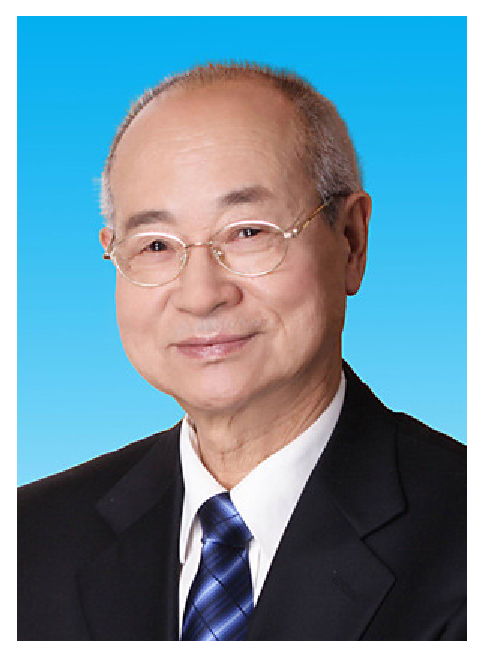
\includegraphics[width=1in,height=1.25in,clip,keepaspectratio]{fig/minyinghua}}]{Yinghua Min} graduated from mathematics department of Jilin university, Changchun, China in 1962, and completed his graduate study in electrical engineering at China Academy of Railway Sciences, Beijing in 1966, although no degree was issued at that time in P.R.China.  He has visited Stanford and other universities in the US for years since 1981.  He is now a professor of Computer science at Institute of Computing Technology, Chinese Academy of Sciences, Beijing, the associate editor-in-chief of ��Journal of Computer Science and Technology��, Honored Chair of technical committee on fault-tolerant computing, China Computer Federation.  He is also a member of the expert committee of the SOC project for the National Natural Science Foundation of China.  He published 230 technical papers, and 4 books, and received the Natural Science award three times from the Chinese Academy of Sciences.  He served as general chairs and program chairs for a number of IEEE symposia and workshops. He is now Co-Chair of the Dragon Star program, a program for US professors to help the People��s Republic of China (PRC) to improve its graduate education in Computer Science and Engineering. He is a Fellow of IEEE, a member of ACM, and a Golden Core Member of IEEE Computer Society.  His current research interests include electronic testing, dependable computing, and networking.
\end{IEEEbiography}

\begin{IEEEbiography}[{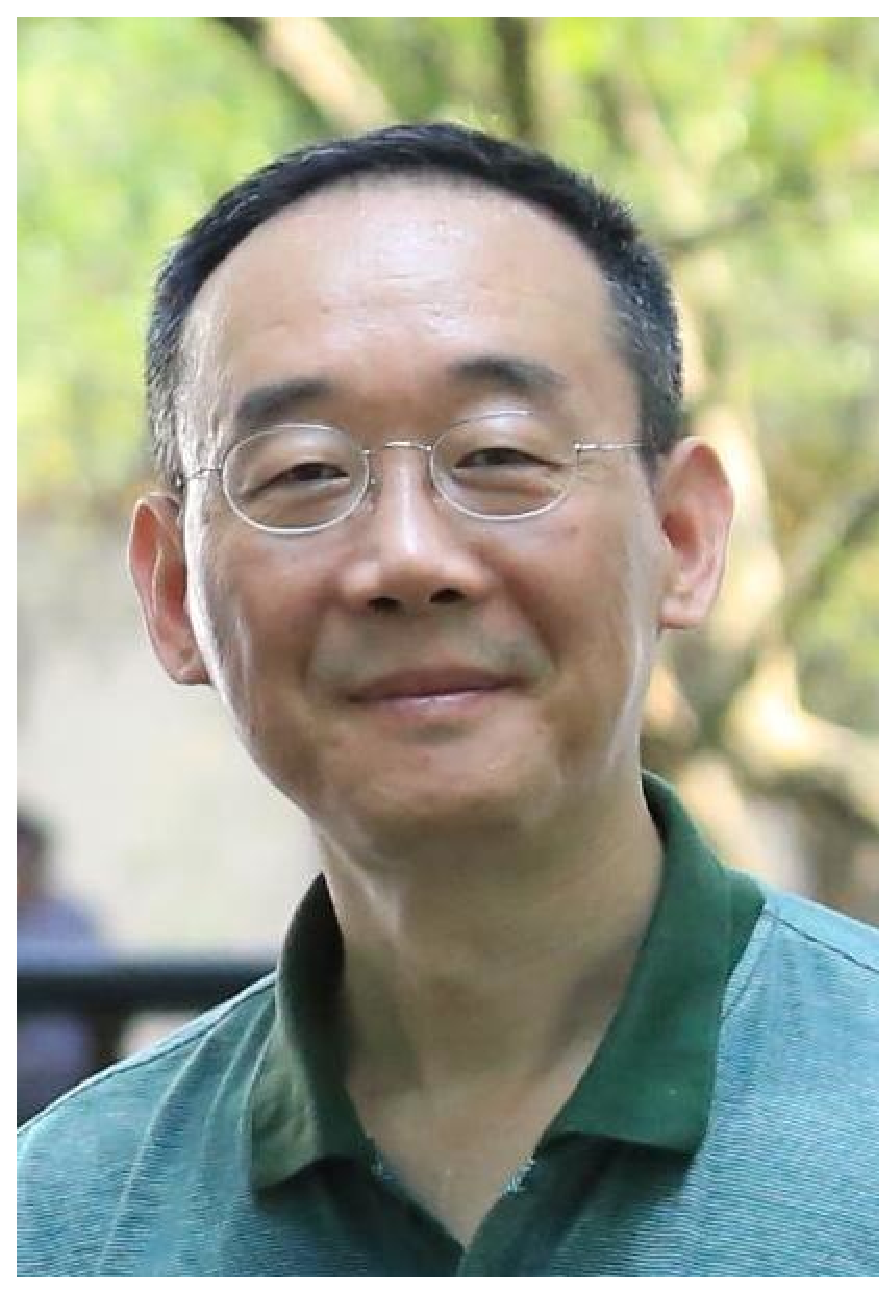
\includegraphics[width=1in,height=1.25in,clip,keepaspectratio]{fig/KeqinLi}}]{Keqin Li} is a SUNY Distinguished Professor of computer science.
His current research interests include
parallel computing and high-performance computing,
distributed computing,
energy-efficient computing and communication,
heterogeneous computing systems,
cloud computing,
big data computing,
CPU-GPU hybrid and cooperative computing,
multicore computing,
storage and file systems,
wireless communication networks,
sensor networks,
peer-to-peer file sharing systems,
mobile computing,
service computing,
Internet of things and cyber-physical systems.
He has published over 400 journal articles, book chapters, and refereed conference papers,
and has received several best paper awards.
He is currently or has served on the editorial boards of
{\em IEEE Transactions on Parallel and Distributed Systems},
{\em IEEE Transactions on Computers},
{\em IEEE Transactions on Cloud Computing},
{\em Journal of Parallel and Distributed Computing}.
He is an IEEE Fellow.
\end{IEEEbiography}
\vspace{-30pt}
\begin{IEEEbiography}[{
\includegraphics[width=1in,height=1.25in,clip,keepaspectratio]{fig/gaogangxie}}]{Gaogang Xie}
received his B.S. degree in Physics, M.S. degree and Ph.D. degree in computer science all from Hunan University respectively in 1996, 1999 and 2002. He is currently a Professor and Director of Network Technology Research Center with the Institute of Computing Technology (ICT), Chinese Academy of Sciences (CAS), Beijing, China. His research interests include Internet architecture, packet processing and forwarding, and Internet measurement.
\end{IEEEbiography}
\vspace{-30pt}

\end{document}
